% !TEX root = ../main.tex
\chapter{Classless D\&D} \label{ch::classlessdnd}
\DndDropCapLine{A}{n inch away from death, a band of}
fellows barely manages to escape from a bloodthirsty nidhogg.
Worn and weary, they settle against an outcrop of rocks, taking a moment to catch their breath.

Nightfall comes all too fast, and they improvise a campfire to keep them warm during the night.
Just as they begin their well-deserved rest, they feel an unsettling rumbling beneath their feet.
What they originally thought was a strange-looking rock starts moving, revealing itself to be a troll.
Tired they scramble for arms, a gat grabbing their mace, and an ird her trusty quarterstaff.

\subsection*{Call to Adventure}
    Adventurers leave home as any person would, picking up an assortment of skills and feats on the road.
    Unskilled and untrained, they take their time to become experts in what they do.
    Lest they become prey to a savage beast or an opportunist bandit.

% \begin{tikzpicture}[remember picture,overlay]
%     \node[anchor=south, yshift=-0.10cm] at (current page.south) {\includegraphics[width=\pdfpagewidth]{06classless/img/00jungle_adventure}};
% \end{tikzpicture}

\subsection*{Creating a character}
    Your first step in playing is creating a character of your own.
    You choose a kin, which will determine their physical characteristics and provide them with a set of traits.
    Then, you choose a background, which describes what they did before joining the adventuring life and provides them with one feature.
    Additionally, your character's kin and background will give them access to a specific set of feats.
    You also invent the personality, appearance, and backstory of your character.

    \subsubsection{Ability Scores}
        After choosing your character's kin and background, it's time to generate their ability scores randomly.
        Roll four d6s and record the total of the highest three dice on a piece of scratch paper.
        Do this five more times, so that you have six numbers.

        Now take your six numbers and write each beside one of your character's six abilities to assign scores to Strength, Dexterity, Constitution, Intelligence, Wisdom, and Charisma.
        Afterward, make any changes to your ability scores as a result of your kin choice.

        After assigning your ability scores, determine your ability modifiers.
        This is done by subtracting 10 from the ability score and then dividing the result by 2 (round down).
        Write the modifier next to each of your scores.

    \subsubsection{Hit Points and Hit Dice}
        On creation, your character has a number of hit points equal to 8 + their Constitution modifier.
        Upon leveling up, roll a d8 and add the number rolled + your character's Constitution modifier to their hit point pool.
        Alternatively, you can forgo this roll and simply add 5 + your character's Constitution modifier.

        Your character has a number of hit dice equal to their level.
        By default all these hit dice are d8s, but they can be improved (or worsened) by taking relevant major character improvements, which are described in a following section.

    \subsubsection{Proficiency Levels}
        Instead of having one particular proficiency bonus, your character has specific proficiency levels in different skills, proficiencies, and saving throws.
        Proficiency levels in skills and proficiencies are gained via feats, while in saving throws they are gained at specific levels, as is listed in the Character Progression Table.

        There are five proficiency levels:
        \subparagraph{Untrained} Completely unskilled in the practice, you have no proficiency bonus.
        \subparagraph{Competent} Some basic experience gives you a +2 proficiency bonus.
        \subparagraph{Skilled} Practice makes perfect, you have a +4 proficiency bonus.
        \subparagraph{Expert} A fully realized professional, you have a +6 proficiency bonus.
        \subparagraph{Legendary} Your skill is lauded, and your crafts acclaimed.
        You have a +12 proficiency bonus.

    % NOTE: It might be cool to find a way to make this look more like the official class summary tables.
    \begin{DndTable}[width=\linewidth, header=Character Progression Table]{ccl}
        \textbf{Level} & \textbf{Required FP} & \textbf{Feature} \\
        1              & 0                    & 2 Saving Throw Improvements \\
        2              & 1                    & Ability Score Improvement \\
        3              & 2                    & Major Character Advancement \\
        4              & 3                    & Ability Score Improvement \\
        5              & 5                    & Saving Throw Improvement \\
        6              & 7                    & Ability Score Improvement \\
        7              & 9                    & - \\
        8              & 11                   & Ability Score Improvement \\
        9              & 13                   & Saving Throw Improvement \\
        10             & 15                   & Ability Score Improvement \\
        11             & 18                   & Major Character Advancement \\
        12             & 21                   & Ability Score Improvement \\
        13             & 24                   & Saving Throw Improvement \\
        14             & 27                   & Ability Score Improvement \\
        15             & 30                   & - \\
        16             & 34                   & Ability Score Improvement \\
        17             & 39                   & Saving Throw Improvement \\
        18             & 44                   & Ability Score Improvement \\
        19             & 51                   & Major Character Advancement \\
        20             & 60                   & Ability Score Improvement
    \end{DndTable}

% !TEX root = ../main.tex
\section{Beyond First Level} \label{ssec::beyondfirstlevel}
\DndDropCapLine{W}{ith one heavy loss, the group}
dispatches the fearsome troll.
They perform a small funerary ritual, to then finally get some rest.
Beaten and tired, they learned their lesson for the day.

% TODO: Add more flavor text or add stuff here and there to fill the page.

\thispagestyle{empty}
\begin{tikzpicture}[remember picture,overlay]
    \node[anchor=south, yshift=-0.10cm] at (current page.south) {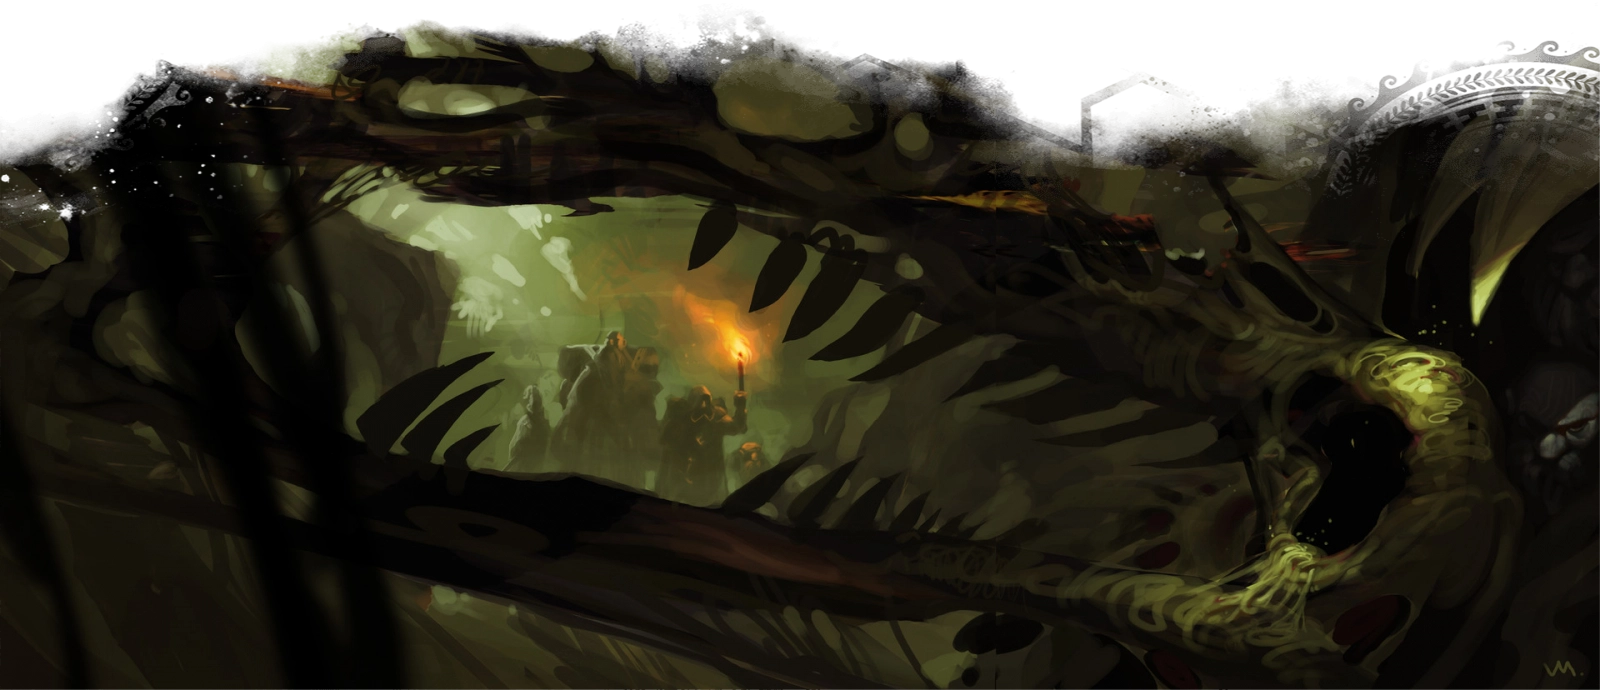
\includegraphics[width=\pdfpagewidth]{06classless/img/10jungle_adventure}};
\end{tikzpicture}

\subsubsection{Experience}
    What is learned by your character during the game is measured by Experience Points (XP).
    After you finish playing, talk about the session with the whole group and discuss what happened.
    Read the questions in the table below.
    For each of them that you can reply ``yes'' to, your character gets one XP.

    \begin{itemize}
        \item Did you participate in the session?
        \item Did you travel to a new location?
        \item Did you defeat one or more creatures?
        \item Did you loot treasure?
        \item Did you complete a quest?
        \item Did you solve a conflict?
        \item Did you make a new friend, ally, or enemy?
        \item Did you help another PC?
        \item Did your ideals, bonds, or flaws affect any of your decisions during the session?
        \item Did you perform any action related to your kin, background, or origin?
        \item Did you perform an extraordinary action of some kind?
    \end{itemize}

    In case of any discussion or disagreement, the DM always has the last word.
    Additional XP may be awarded when specific story milestones are achieved, but this too is left to the discression of the DM.

    \newpage

\subsubsection{Feat Points}
    As your character adventures, they will gain \textbf{Feat Points} (FP).
    Feat points are spent to buy feats, which can only be done as part of a long rest.
    You can buy multiple feats in one long rest.
    Feats either increase your proficiency level at a skill or a proficiency, or they include a useful feature.

    When you reach 10 XP, reset your XP counter and add one FP, keeping the remaining XP.
    Feat points are used to learn new feats, which include either an increase in a proficiency level or a feature.

    You don't need to spend FP right after earning it, you can save as many as you want for as long as you need.
    The full list of feats starts in the next page.

\subsubsection{Leveling Up}
    As your character gains feat points they will gain levels, acquiring hit dice, improving their ability scores and saving throw proficiencies, and gaining major character advancements.
    \begin{itemize}
        \item Ability Score Improvements allow you to increase one of you ability scores by 1.
        \item Saving Throw Improvements increase your level of proficiency on a saving throw of your choice by 1.
        As usual, you cannot increase your level of proficiency on a saving throw beyond Expert.
        \item Major Character Advancements are character-defining improvements which include hit dice upgrades, combat styles, and proficiency improvements.
        They are listed in page \pageref{sec::majorcharacterimprovements}.
    \end{itemize}

    When your Constitution modifier increases by 1, your hit point maximum increases by 1 for each level you have attained.
    The same effect happens if you improve your hit dice.
    Similarly, you decrease your hit point maximum by 1 if you worsen your hit dice.

    \newpage

% % !TEX root = ../main.tex
\section{Major Character Improvements} \label{sec::majorcharacterimprovements}
% Fighting style
% Spellcasting style
% Two Expert proficiencies turned to legendary
% Hit Dice upgrade
Upon reaching levels 3, 11, and 19, your character gains Major Character Advancements.

% % !TEX root = ../main.tex
\section{Feats}

% TODO: Consider changing the ``relevant ability score or skill'' to just Intelligence.
%       This would give more relevance to the skill in classes that don't actively use it.
%       Discuss with Hernán.

% TODO: Add the explanation: ``unless specified otherwise, a feat can only be learned once''.

% TODO: Write list of Fighting Styles and ``Casting Styles'' (Based on this: https://standsinthefire.com/2016/05/31/dd-5e-magical-styles/).
% TODO: Combat maneuvers, metamagic options and other **don't have a point system associated to them**. They simply add effects to attacks or spellcasting by using one additional action!
% TODO: Write Combat Maneuvers section.
% TODO: Write list of Metamagic Options.

\subsubsection{Feat Name}
\small{\textcolor{gray}{Relevant Ability Score or Skill}}

\normalsize
Description.
\paragraph{REQUIREMENTS} Other ranks that need to be attained before attaining this one.
Left blank if feat doesn't require anything.

\begin{table*}[b]%
    \begin{DndTable}[width=\linewidth, header=General Feats]{clXX} \label{feat::generalfeats}
        \textbf{Page} & \textbf{Name} & \textbf{Tags} & \textbf{Requirements} \\
        \pageref{feat::acrobat} & Acrobat & acrobatics & - \\
        \pageref{feat::actor} & Actor & performance & Performer 3 \\
        \pageref{feat::aerialist} & Aerialist & acrobatics & Acrobat 3 \\
        \pageref{feat::animalhandler} & Animal Handler & animal handling & - \\
        \pageref{feat::armedfighter} & Armed Fighter & simple weapons & - \\
        \pageref{feat::armorbreaker} & Armor Breaker & martial weapons, medium-haft & Hammer Adept 2 and Heavily Armored 1 \\
        \pageref{feat::athlete} & Athlete & athletics & - \\
        \pageref{feat::axeadept} & Axe Adept & martial weapons, medium-haft & Armed Fighter 2 \\
        \pageref{feat::ballandchainmaster} & Ball and Chain Master & martial weapons, insight & Flail Adept 2 and Insightful 2 \\
        \pageref{feat::bentblademaster} & Bent Blade Master & martial weapons, swords, sleight of hand & Curved Sword Adept 2 and Quick Fingers 2
    \end{DndTable}
\end{table*}

\begin{table*}[b]%
    \begin{DndTable}[width=\linewidth, header=Kin Feats]{clXX} \label{feat::kinfeats}
        \textbf{Page} & \textbf{Name} & \textbf{Tags} & \textbf{Requirements} \\
    \end{DndTable}
\end{table*}

\begin{table*}[b]%
    \begin{DndTable}[width=\linewidth, header=Artisan Feats]{clXX}
        \textbf{Page} & \textbf{Name} & \textbf{Tags} & \textbf{Requirements} \\
    \end{DndTable}
\label{feat::artisanfeats}
\end{table*}

\begin{table*}[b]%
    \begin{DndTable}[width=\linewidth, header=Injury Feats]{clXX} \label{feat::injuryfeats}
        \textbf{Page} & \textbf{Name} & \textbf{Tags} & \textbf{Requirements} \\
    \end{DndTable}
\end{table*}

\subsection*{Feats}
% !TEX root = ../main.tex
\subsubsection{Acrobat} \label{feat::acrobat}
\small{\textcolor{gray}{Acrobatics}}

\normalsize
You've had an exceptional flexibility from a very young age.
By regular training you maintain this ability, aware of its usefulness in your adventuring life.
\paragraph{RANK 1} You are proficient with the Acrobatics skill.
\paragraph{RANK 2} You can make a running long jump or a running high jump after moving only 1.5 meters on foot, rather than 3 meters.
\paragraph{RANK 3} Moving through difficult terrain costs you no extra movement.

% ============================================================================== %
\subsubsection{Actor} \label{feat::actor}
\small{\textcolor{gray}{Performer}}

\normalsize
You master performance so that you can command any stage.
\paragraph{REQUIREMENTS} Performer 3.
\paragraph{RANK 1} You double your proficiency modifier in the Performance skill.
\paragraph{RANK 2} You have advantage on Charisma (Deception) and Charisma (Performance) checks when trying to pass yourself off as a different person.
\paragraph{RANK 3} Increase your Charisma score by 1, to a maximum of 20.

% ============================================================================== %
\subsubsection{Aerialist} \label{feat::aerialist}
\small{\textcolor{gray}{Acrobatics}}

\normalsize
High above the ground, you defy falls to earth on a daily basis.
\paragraph{REQUIREMENTS} Acrobat 3.
\paragraph{RANK 1} You double your proficiency modifier in the Acrobatics skill.
\paragraph{RANK 2} Your walking speed increases by 1.5 meters.
Additionally, you gain a climbing speed and a swimming speed equal to your walking speed.
\paragraph{RANK 3} You learn the Light as a Feather technique.

% ============================================================================== %
\subsubsection{Animal Handler} \label{feat::animalhandler}
\small{\textcolor{gray}{Animal Handling}}

\normalsize
Ever since you were a kid, you've always surrounded yourself with animals, pets or otherwise.
Animals are calmer when they're around you, and you yourself get the same feeling when around them.
\paragraph{RANK 1} You are proficient with the Animal Handling skill.
\paragraph{RANK 2} Animals naturally trust you, and you don't need to perform any check to calm an animal or monster that is not already violent toward you.
\paragraph{RANK 3} You learn the Beast Command technique.

% ============================================================================== %
\subsubsection{Armed Fighter} \label{feat::armedfighter}
\small{\textcolor{gray}{Strength or Dexterity}}

\normalsize
No one learned how to use a sword without first swinging a stick.
\paragraph{RANK 1} You are proficient with simple weapons.
\paragraph{RANK 2} You can attack twice, instead of once, whenever you take the Attack action on your turn.
\paragraph{RANK 3} You learn one technique of your choice between Bonk, Block, Buttstroke, Feint, Lunge, Parry, Pushing Attack, Protect, Quick Draw, Riposte, Rush, Sweep, and Trip.

% ============================================================================== %
\subsubsection{Armor Breaker} \label{feat::armorbreaker}
\small{\textcolor{gray}{Strength}}

\normalsize
You use your extensive knowledge of heavy armor to improve your effectiveness against it, turning your bludgeoning attacks into devastating metal bending strikes.
\paragraph{REQUIREMENTS} Hammer Adept 2 and Heavily Armored 1.
\paragraph{RANK 1} You can use the Bonk technique as an opportunity attack.
\paragraph{RANK 2} When fighting a target with plate armor or natural armor, you get a +2 bonus to your melee attacks with hammers.
\paragraph{RANK 3} You learn the Fell Strike technique.

% ============================================================================== %
\subsubsection{Athlete} \label{feat::athlete}
\small \textcolor{gray}{Athletics}

\normalsize
You begin your day by training, pushing the limits of your body ever so slightly.
\paragraph{RANK 1} You are proficient with the Athletics skill.
\paragraph{RANK 2} When you are prone, standing up uses only 1.5 meters of your movement.
\paragraph{RANK 3} You count as if you were one size larger for the purpose of determining your carrying capacity.

% ============================================================================== %
\subsubsection{Axe Adept} \label{feat::axeadept}
\small{\textcolor{gray}{Strength}}

\normalsize
More than a simple tool, you master the use of axes in combat.
\paragraph{REQUIREMENTS} Armed Fighter 2.
\paragraph{RANK 1} You are proficient with axes.
\paragraph{RANK 2} While wielding an axe, you get advantage on your attack rolls with the Disarm action when forcing your target to drop a shield.
\paragraph{RANK 3} You learn the Rush technique.

% ============================================================================== %
\subsubsection{Ball-and-Chain Master} \label{feat::ballandchainmaster}
\small{\textcolor{gray}{Strength}}

\normalsize
Your increased awareness works in tandem to your flail mastery, allowing you to hit enemies behind obstacles and shields.
\paragraph{REQUIREMENTS} Flail Adept 2 and Insightful 2.
\paragraph{RANK 1} When you use a ball-and-chain, its damage die changes from a d6 to a d8.
\paragraph{RANK 2} When you hit with an opportunity attack using a ball-and-chain, the target must succeed on a Strength saving throw (DC 8 + your proficiency bonus + your Strength modifier) or be knocked prone.
\paragraph{RANK 3} You learn the Shield Sweep technique.

% ============================================================================== %
\subsubsection{Bent Blade Master} \label{feat::bentblademaster}
\small{\textcolor{gray}{Dexterity}}

\normalsize
Your extreme skill with curved swords allows you to cut through flesh with effectiveness and ease.
\paragraph{REQUIREMENTS} Curved Sword Adept 2 and Quick Fingers 2.
\paragraph{RANK 1} While you're wielding at least one curved sword and a creature gets an attack of opportunity on you, they attack with disadvantage.
\paragraph{RANK 2} You get a +2 bonus to your melee weapon attack damage with curved blades.
This extra damage is nullified against targets with chainmail, plate armor, or natural armor.
\paragraph{RANK 3} You learn the Shield Sweep technique.

% ============================================================================== %
\subsubsection{Blade \& Board} \label{feat::bladeandboard}
\small{\textcolor{gray}{Strength}}

\normalsize
You know the perfect balance between defense and attack, making you a formidable foe in melee combat.
\paragraph{REQUIREMENTS} Straight Blade Adept 2 and Shield Training 2, or Axe Adept 2 and Shield Training 2.
\paragraph{RANK 1} When you're wielding a slashing weapon and a shield, you gain a +1 to AC and to your attack damage.
\paragraph{RANK 2} While you're wielding a shield and a creature misses you with a melee attack, you can use your reaction to attack it with a melee attack.
\paragraph{RANK 3} You learn the Bash technique.

% ============================================================================== %
\subsubsection{Blade Breaker} \label{feat::bladebreaker}
\small{\textcolor{gray}{Dexterity}}

\normalsize
You know that the perfect counter against any sword is simply a long pole.
\paragraph{REQUIREMENTS} Staff Fighter 2.
\paragraph{RANK 1} Staves have the Reach property when wielded by you.
\paragraph{RANK 2} You have advantage on the Disarm action and the Parry technique against creatures using any type of sword.
\paragraph{RANK 3} While using a polearm, you can use the Disarm action as your opportunity attack.

% ============================================================================== %
\subsubsection{Blowgun Adept} \label{feat::blowgunadept}
\small{\textcolor{gray}{Dexterity}}

\normalsize
While unconventional, you understand the effectiveness of the blowgun when remaining hidden is of the essence.
\paragraph{REQUIREMENTS} Armed Fighter 1.
\paragraph{RANK 1} You are proficient with blowguns.
\paragraph{RANK 2} You gain a +1 bonus to attack rolls with a blowgun.
Additionally, attacking with a blowgun at long range doesn't impose disadvantage on your ranged weapon attack rolls.
\paragraph{RANK 3} When you hit with a blowgun while hidden, your location is not revealed.

% ============================================================================== %
\subsubsection{Blunt Thrower} \label{feat::bluntthrower}
\small{\textcolor{gray}{Strength}}

\normalsize
You take advantage of the raw practicality of a good hammer, and not even faraway foes can escape the wrath of its face.
\paragraph{REQUIREMENTS} Hammer Adept 2 and Thrown Weapon Master 2.
\paragraph{RANK 1} You don't provoke opportunity attacks when picking weapons up from the floor.
\paragraph{RANK 2} When you hit a creature with an thrown bludgeoning weapon, you divide its moving speed by half (rounded up) during its next turn.
This effect does not stack.
\paragraph{RANK 3} You learn the Hammer Fling technique.

% ============================================================================== %
\subsubsection{Blunt Master} \label{feat::bluntmaster}
\small{\textcolor{gray}{Dexterity}}

\normalsize
Your staff is an extension of your body, and it has become an essential part of your movement and defense.
\paragraph{REQUIREMENTS} Staff Fighter 2 and Unarmed Artist 2.
\paragraph{RANK 1} As a bonus action, you can use your staff to propel yourself into the air, making a high jump up to your Dexterity modifier times 1.5 meters.
Additionally, if you have moved at least 3 meters during this round, you can jump in a straight line up to a distance equal to your Dexterity modifier times 3 meters.
\paragraph{RANK 2} You gain a +1 bonus to your AC while using a staff.
Additionally, if you use the weapon with two hands you gain another +1 bonus to your AC.
\paragraph{RANK 3} You learn the Defensive Stance technique.

% ============================================================================== %
\subsubsection{Bow Adept} \label{feat::bowadept}
\small{\textcolor{gray}{Dexterity}}

\normalsize
While a long list of new ranged weapons have recently appeared, you know that nothing beats the long range of the traditional bow.
\paragraph{REQUIREMENTS} Armed Fighter 2.
\paragraph{RANK 1} You are proficient with bows.
\paragraph{RANK 2} After you successfully hit a target with a melee attack using your bow, that creature can't make opportunity attacks against you until the start of your next turn.
\paragraph{RANK 3} You learn the Quick Draw technique.

% ============================================================================== %
\subsubsection{Buckler Training} \label{feat::bucklertraining}
\small{\textcolor{gray}{Dexterity}}

\normalsize
Small shields are much more than a weaker version of the standard shields.
They allow you to remain mobile while still providing a solid defense against even the fastest assailants.
\paragraph{RANK 1} You gain proficiency with light shields.
\paragraph{RANK 2} In combat, you can don or doff a light shield as the free object interaction of your turn.
\paragraph{RANK 3} You learn the Parry technique.

% ============================================================================== %
\subsubsection{Bullet Tinkerer} \label{feat::bullettinkerer}
\small{\textcolor{gray}{Science}}

\normalsize
Firearm ammunition is near impossible to find or purchase in most parts of Yuadrem.
Due to this, learning how to craft it yourself is an essential aspect for using firearms.
\paragraph{REQUIREMENTS} Musket Adept 2 and Educated 2, or Pistol Adept 2 and Educated 2.
\paragraph{RANK 1} You can craft ammunition using a set of Tinker's Tools at half the cost.
\paragraph{RANK 2} If you roll a misfire, you can use your reaction to roll a d20 with disadvantage.
If the number rolled is higher than the weapon's misfire score, the weapon does not misfire.
\paragraph{RANK 3} You learn the Violent Shot technique.

% ============================================================================== %
\subsubsection{Cognizant} \label{feat::cognizant}
\small{\textcolor{gray}{History}}

\normalsize
From background or perchance you've been given a privileged access to books and teaching thorough your life.
\paragraph{RANK 1} You are proficient with the History skill.
\paragraph{RANK 2} You have advantage on any Intelligence (History) checks to recall information of your kin and your country of origin.
\paragraph{RANK 3} You learn the Wizened Advice technique.

% ============================================================================== %
\subsubsection{Combat Improviser} \label{feat::combatimproviser}
\small{\textcolor{gray}{Strength or Dexterity}}

\normalsize
Anything can be your weapon.
If you can grab it, you can swing it.
\paragraph{REQUIREMENTS} Armed Fighter 1.
\paragraph{RANK 1} You are proficient with improvised weapons.
An improvised weapon is anything that is somewhat similar to a simple weapon.
\paragraph{RANK 2} After rolling for initiative, you make your first attack with an improvised weapon at advantage.
\paragraph{RANK 3} You learn one technique of your choice between Bonk, Block, Buttstroke, Feint, Lunge, Parry, Pushing Attack, Protect, Quick Draw, Riposte, Rush, Sweep, and Trip.

% ============================================================================== %
\subsubsection{Covered Shooter} \label{feat::coveredshooter}
\small{\textcolor{gray}{Dexterity}}

\normalsize
You know that stealth and range go hand in hand.
\paragraph{REQUIREMENTS} Bow Adept 2 and Sly 2.
\paragraph{RANK 1} If you miss with a ranged attack with a bow or thrown weapon while hidden, the attack doesn't reveal your location, and you remain hidden.
\paragraph{RANK 2} You can treat ranged attack damage die rolls of 1 as 2.
\paragraph{RANK 3} You learn or improve the Sneak Attack technique.

% ============================================================================== %
\subsubsection{Crossbow Adept} \label{feat::crossbowadept}
\small{\textcolor{gray}{Dexterity}}

\normalsize
You are learned with the use of crossbow, and can use it proficiently both for hunting and combat.
\paragraph{REQUIREMENTS} Armed Fighter 2.
\paragraph{RANK 1} You are proficient with crossbows.
\paragraph{RANK 2} You can change the loading quality of crossbows to reloading.
% You can ignore the loading quality of crossbows.
\paragraph{RANK 3} You learn the Buttstroke technique.

% ============================================================================== %
\subsubsection{Crossbow Expert} \label{feat::crossbowexpert}
\small{\textcolor{gray}{Dexterity}}

\normalsize
While muskets and pistols have largely replaced the old weapons of warfare, you prefer a weapon that won't blow up on your hand every so often.
\paragraph{REQUIREMENTS} Crossbow Adept 2 and Quick Fingers 2.
\paragraph{RANK 1} Being within 1.5 meters of a hostile creature doesn't impose disadvantage on your ranged attack rolls.
Additionally, you don't provoke attacks of opportunity when using the Attack action with a ranged weapon when within the reach of a creature.
\paragraph{RANK 2} You get a +2 bonus to damage rolls when attacking a creature within 1.5 meters of you with a crossbow.
\paragraph{RANK 3} You learn the Prepared Shot technique.

% ============================================================================== %
\subsubsection{Crusher} \label{feat::crusher}
\small{\textcolor{gray}{Strength}}

\normalsize
You are practiced in the art of crushing your enemies.
\paragraph{REQUIREMENTS} Proficiency with at least two martial bludgeoning weapon types.
\paragraph{RANK 1} Once per turn, when you hit a creature with an attack that deals bludgeoning damage, you can move it 1.5 meters to an unoccupied space, provided that the target is no more than one size larger than you.
\paragraph{RANK 2} Increase your Strength by 1, to a maximum of 20.
\paragraph{RANK 3} You learn the Whack technique.

% ============================================================================== %
\subsubsection{Curved Sword Adept} \label{feat::curvedswordadept}
\small{\textcolor{gray}{Strength or Dexterity}}

\normalsize
You forfeited the piercing capacity of the straight blades to maximize your deadliness against the unarmored.
\paragraph{REQUIREMENTS} Armed Fighter 2.
\paragraph{RANK 1} You are proficient with curved swords.
\paragraph{RANK 2} While wielding a curved sword, you get advantage on your attack rolls with the Disarm action when forcing your target to drop a weapon.
\paragraph{RANK 3} You learn the Parry technique.

% ============================================================================== %
\subsubsection{Cutthroat} \label{feat::cutthroat}
\small{\textcolor{gray}{Dexterity}}

\normalsize
A master at concealing your dagger, you act quick and strike hard in combat.
\paragraph{REQUIREMENTS} Dagger Savant 2.
\paragraph{RANK 1} You have advantage on any check to conceal a small weapon on your person.
\paragraph{RANK 2} You gain a +2 bonus to initiative. % when wielding a light weapon.
\paragraph{RANK 3} You gain or improve the Sneak Attack technique.

% ============================================================================== %

% !TEX root = ../main.tex
\subsubsection{Dagger Savant} \label{feat::daggersavant}
\small{\textcolor{gray}{Dexterity}}

\normalsize
You wield the lightest of blades with the deadliest of skills.
\paragraph{REQUIREMENTS} Armed Fighter 1.
\paragraph{RANK 1} You can perform one melee attack with a dagger as part of a Grapple, Escape a Grapple, Overrun, or Tumble action.
\paragraph{RANK 2} You gain or improve the Sneak Attack technique.
\paragraph{RANK 3} You learn the Riposte technique.

% ============================================================================== %
\subsubsection{Defensive Duelist} \label{feat::defensiveduelist}
\small{\textcolor{gray}{Dexterity}}

\normalsize
A master of the buckler, you have learned to use it as an addition to your main weapon.
\paragraph{REQUIREMENTS} Buckler Training 2.
\paragraph{RANK 1} When you use the Parry technique, you can roll a d8 instead of a d6 when increasing your AC.
\paragraph{RANK 2} When fighting with a one-handed melee weapon and a light shield, you can add half your shield's AC (rounded up) to the weapon's attack damage.
\paragraph{RANK 3} When you use your Parry technique and the attacking creature misses, you can use the Disarm action against it as part of your reaction.

% ============================================================================== %
\subsubsection{Deft Explorer} \label{feat::deftexplorer}
\small{\textcolor{gray}{Nature}}

\normalsize
You are an unsurpassed explorer, using your uncanny knowledge of nature to understand and survive in any environment.
\paragraph{REQUIREMENTS} Naturalist 3.
\paragraph{RANK 1} You double your proficiency modifier in the Nature skill.
\paragraph{RANK 2} By almost supernatural perception, you can sense the presence of poisons and poisonous creatures within 9 meters of you.
\paragraph{RANK 3} Increase your Intelligence score by 1, to a maximum of 20.

% ============================================================================== %
\subsubsection{Detective} \label{feat::detective}
\small{\textcolor{gray}{Investigation}}

\normalsize
You excel at rooting out secrets and unraveling mysteries.
\paragraph{REQUIREMENTS} Inquisitive 3.
\paragraph{RANK 1} You double your proficiency modifier in the Investigation skill.
\paragraph{RANK 2} You have a +5 bonus to your passive intelligence (Investigation) score.
\paragraph{RANK 3} Increase your Intelligence score by 1, to a maximum of 20.

% ============================================================================== %
\subsubsection{Dual Wielder} \label{feat::dualwielder}
\small{\textcolor{gray}{Dexterity}}

\normalsize
You master fighting with two weapons.
\paragraph{REQUIREMENTS} Dexterity 13. Armed Fighter 2.
\paragraph{RANK 1} When you engage in two-weapon fighting, you can add your ability modifier to the damage of the second attack.
\paragraph{RANK 2} You can draw or stow two one-handed weapons when you would normally be able to draw or stow only one.
\paragraph{RANK 3} You learn the Lock technique.

% ============================================================================== %
\subsubsection{Educated} \label{feat::educated}
\small{\textcolor{gray}{Science}}

\normalsize
From background or perchance you've been given a privileged access to books and teaching thorough your life.
You have an advanced understanding of the natural laws of the world.
\paragraph{RANK 1} You are proficient with the Science skill.
\paragraph{RANK 2} You have advantage on the Identify a Spell action.
\paragraph{RANK 3} You have an intuitive understanding of how to use all sorts of machinery, and can operate siege weapons and heavy machines without performing any ability checks.

% ============================================================================== %
\subsubsection{Empathetic} \label{feat::empathetic}
\small{\textcolor{gray}{Insight}}

\normalsize
You possess keen insight into how other people think and feel.
\paragraph{REQUIREMENTS} Insightful 3.
\paragraph{RANK 1} You double your proficiency modifier in the Insight skill.
\paragraph{RANK 2} You learn the Uncanny Insight technique.
\paragraph{RANK 3} Increase your Wisdom score by 1, to a maximum of 20.

% ============================================================================== %
\subsubsection{Estoc Master} \label{feat::estocmaster}
\small{\textcolor{gray}{Dexterity}}

\normalsize
A master of thrust, you prefer to focus only on piercing and abandon the slashing capabilities of the rapier.
\paragraph{REQUIREMENTS} Light Sword Adept 2.
\paragraph{RANK 1} Whenever you miss with a melee weapon attack, you can use your reaction to reroll that attack if you're wielding an estoc.
\paragraph{RANK 2} You can attack twice instead of once when you use your reaction to attack with the Riposte technique.
\paragraph{RANK 3} While wielding an estoc, you can attack one additional time when you use the attack action.

% ============================================================================== %
\subsubsection{Far Thruster} \label{feat::farthruster}
\small{\textcolor{gray}{Strength or Dexterity}}

\normalsize
You take advantage of your long weapon to keep your distance from foes.
\paragraph{REQUIREMENTS} Halberd Adept 2 and Spear Adept 2.
\paragraph{RANK 1} After successfully attacking a creature, you can use the Shove action as a bonus action.
\paragraph{RANK 2} You gain a +2 to your attack rolls made with a polearm against a creature larger than you.
\paragraph{RANK 3} You learn the Extend Reach technique.

% ============================================================================== %
\subsubsection{Fearsome} \label{feat::fearsome}
\small{\textcolor{gray}{Intimidation}}

\normalsize
You become fearsome to others, and people are scared to even talk about you.
\paragraph{REQUIREMENTS} Menacing 3.
\paragraph{RANK 1} You double your proficiency modifier in the Intimidation skill.
\paragraph{RANK 2} You learn the Demoralize technique.
\paragraph{RANK 3} Increase your Charisma score by 1, to a maximum of 20.

% ============================================================================== %
\subsubsection{Fell Hand} \label{feat::fellhand}
\small{\textcolor{gray}{Strength}}

\normalsize
You are an expert with the greatclub, and can use its raw power to pancake even the hardiest foes.
\paragraph{REQUIREMENTS} Hammer Adept 2.
\paragraph{RANK 1} When you use a greatclub, its damage die changes from a d8 to a d10.
\paragraph{RANK 2} Whenever you miss with a melee attack using a greatclub, the target takes bludgeoning damage equal to your Strength modifier (minimum of 2).
\paragraph{RANK 3} When your target fails its saving throw against your Bonk technique, it also falls prone.

% ============================================================================== %
\subsubsection{Fencer} \label{feat::fencer}
\small{\textcolor{gray}{Dexterity}}

\normalsize
More than a mere combatant, you are able to dance in the battlefield when using your light blades.
\paragraph{REQUIREMENTS} Light Sword Adept 2 and Performer 2.
\paragraph{RANK 1} You gain a +1 to melee attack rolls and AC when only one creature is within 5 feet of you.
\paragraph{RANK 2} When you use your Parry technique and the attacking creature misses, you can use the Riposte technique without using your reaction.
\paragraph{RANK 3} You learn the Focus Strikes technique.

% ============================================================================== %
\subsubsection{Firearm Specialist} \label{feat::firearmspecialist}
\small{\textcolor{gray}{Dexterity}}

\normalsize
You are particularly well at combat with pistols, and are a shining example of this new weapon's viability in combat.
\paragraph{REQUIREMENTS} Pistol Adept 2.
\paragraph{RANK 1} You can reload any weapon as a bonus action.
\paragraph{RANK 2} If you are using a pistol in one hand and nothing on the other, you get a +2 bonus to your ranged weapon attacks with it.
\paragraph{RANK 3} You learn the Rapid Repair technique.

% ============================================================================== %
\subsubsection{Flail Adept} \label{feat::flailadept}
\small{\textcolor{gray}{Strength or Dexterity}}

\normalsize
The flail is a tricky weapon to use, but you have spent countless hours mastering it.
\paragraph{REQUIREMENTS} Armed Fighter 2.
\paragraph{RANK 1} You are proficient with flails.
\paragraph{RANK 2} When wielding flails, enemies provoke opportunity attacks from you when they enter your reach.
\paragraph{RANK 3} You learn the Sweep technique.

% ============================================================================== %

% !TEX root = ../main.tex
\subsubsection{Giant Slayer} \label{feat::giantslayer}
\small{\textcolor{gray}{Strength}}

\normalsize
Partaking or not in Krudzal's Eternal War, you use your incredible strength to wield their massive weapons.
\paragraph{REQUIREMENTS} Strength 16. Great Weapon User 2.
\paragraph{RANK 1} You are able to use Krudzal's giant-slayers.
\paragraph{RANK 2} You gain a +1 bonus to damage rolls with weapons with the Great property.
\paragraph{RANK 3} When fighting with a melee giant-slayer, you can attack up to three creatures in range with one attack.
Additionally, you can reload the hand ballista as a bonus action instead of an action.

% ============================================================================== %
\subsubsection{Glaive Master} \label{feat::glaivemaster}
\small{\textcolor{gray}{Dexterity}}

\normalsize
Different than the common polearm, you know how deadly a glaive can be in capable hands.
\paragraph{REQUIREMENTS} Halberd Adept 2.
\paragraph{RANK 1} When you use a glaive, its damage die changes from a d10 to a d12.
\paragraph{RANK 2} The glaive has the finesse property for you.
\paragraph{RANK 3} When you miss an attack, you can attempt to strike your enemy with the rondel of your glaive as a free action.
On a hit, the target takes 1d4 + your Strength modifier bludgeoning damage.
You can do this once per turn.

% ============================================================================== %
\subsubsection{Grappler} \label{feat::grappler}
\small{\textcolor{gray}{Strength}}

\normalsize
You've developed the skills necessary to hold your own in close-quarters grappling.
\paragraph{REQUIREMENTS} Pugilist 2.
\paragraph{RANK 1} You have advantage on attack rolls against creatures you are grappling.
\paragraph{RANK 2} You benefit from three-quarters cover while you grapple a creature of a size equal or greater than yours.
\paragraph{RANK 3} You learn the Pin technique.

% ============================================================================== %
\subsubsection{Great Weapon User} \label{feat::greatweaponuser}
\small{\textcolor{gray}{Strength}}

\normalsize
You've learned to put the weight of a weapon to your advantage, letting its momentum empower your strikes.
\paragraph{REQUIREMENTS} Strength 13. Armed Fighter 2.
\paragraph{RANK 1} You can use weapons with the great property.
Some of these, like the zweihander and the greataxe, also require you to have proficiency with the corresponding weapon type.
\paragraph{RANK 2} On your turn, when you score a critical hit with a melee weapon or reduce a creature to 0 hit points with one, you can make one melee weapon attack as a bonus action.
\paragraph{RANK 3} You learn the Reckless Strike technique.

% ============================================================================== %
\subsubsection{Greatshield Training} \label{feat::greatshieldtraining}
\small{\textcolor{gray}{Strength}}

\normalsize
When it comes to protecting your life or that of others, you know that size matters.
\paragraph{REQUIREMENTS} Shield Training 1.
\paragraph{RANK 1} You gain proficiency with heavy shields
\paragraph{RANK 2} Creatures standing behind you get three-fourths cover against ranged attacks.
\paragraph{RANK 3} You learn the Protect technique.

% ============================================================================== %
\subsubsection{Gunner} \label{feat::gunner}
\small{\textcolor{gray}{Dexterity}}

\normalsize
Being a new breed of weapon, firearms are constantly subject to change and refinement.
New weapons appear by the minute, and you are an expert at experimenting with them.
\paragraph{REQUIREMENTS} Pistol Adept 2 and Musket Adept 2.
\paragraph{RANK 1} As long as you can examine the weapon for 30 seconds, you are proficient with any kind of firearm, even if it is new or experimental.
\paragraph{RANK 2} Your firearm attacks score a critical hit on a roll of 19-20.
\paragraph{RANK 3} You learn the Reckless Shot technique.

% ============================================================================== %
\subsubsection{Haggler} \label{feat::haggler}
\small{\textcolor{gray}{Persuasion}}

\normalsize
Your abilities at haggling and persuading are known in your local markets, and you are both feared and revered by merchants and traders.
\paragraph{REQUIREMENTS} Persuasive 3.
\paragraph{RANK 1} You double your proficiency modifier in the Persuasion skill.
\paragraph{RANK 2} Your well-honed haggling skills allow you to shave off 10\% off the price of anything, even if you fail a Charisma (Persuasion) check.
\paragraph{RANK 3} Increase your Charisma score by 1, to a maximum of 20.

% ============================================================================== %
\subsubsection{Halberd Adept} \label{feat::halberdadept}
\small{\textcolor{gray}{Strength or Dexterity}}

\normalsize
You know that both farmers and nobles use halberds as their weapon of choice for a reason.
\paragraph{REQUIREMENTS} Armed Fighter 2 and Staff Fighter 2.
\paragraph{RANK 1} You are proficient with the many varieties of halberds.
\paragraph{RANK 2} When a creature within 1.5 meters of you makes an attack against a target other than you, you can use your reaction to make a melee weapon attack against the attacking creature.
\paragraph{RANK 3} You learn the Trip technique.

% ============================================================================== %
\subsubsection{Hammer Adept} \label{feat::hammeradept}
\small{\textcolor{gray}{Strength}}

\normalsize
If a hammer will do, why complicate things?
\paragraph{REQUIREMENTS} Armed Fighter 2.
\paragraph{RANK 1} You gain proficiency with hammer weapons.
\paragraph{RANK 2} If you use the Help action to aid an ally's melee attack while you're wielding a hammer weapon, you knock the target's shield aside momentarily.
In addition to the ally gaining advantage on the attack roll, the ally gains a bonus to the roll equal to the shield's AC bonus.
\paragraph{RANK 3} You learn the Bonk technique.

% ============================================================================== %
\subsubsection{Hand Crossbow Master} \label{feat::handcrossbowmaster}
\small{\textcolor{gray}{Dexterity}}

\normalsize
You can equip, load, and shoot a hand crossbow in an instant, and with deadly effect.
\paragraph{REQUIREMENTS} Crossbow Adept 2.
\paragraph{RANK 1} You can reload a hand crossbow or one-handed firearm without having a free hand.
\paragraph{RANK 2} You can ignore the loading (or reloading) quality of hand crossbows.
\paragraph{RANK 3} You can don and you can doff a one-handed ranged weapon as your free object interaction during your turn.
The two actions don't need to be done in tandem - for example, you can don a hand crossbow, shoot an arrow, and doff it during one turn.

% ============================================================================== %
\subsubsection{Heavily Armored} \label{feat::heavilyarmored}
\small{\textcolor{gray}{Strength}}

\normalsize
You are trained to use heavy armor.
\paragraph{REQUIREMENTS} Moderately Armored 1.
\paragraph{RANK 1} You gain proficiency with heavy armor.
\paragraph{RANK 2} Equipped heavy armor and metal accessories only add half their weight to your encumbrance.
\paragraph{RANK 3} Increase your Strength by 1, to a maximum of 20.

% ============================================================================== %
\subsubsection{Heavy Armor Master} \label{feat::heavyarmormaster}
\small{\textcolor{gray}{Strength}}

\normalsize
You can use your armor to deflect strikes that would easily kill others.
\paragraph{REQUIREMENTS} Heavily Armored 2 and Athletics 2.
\paragraph{RANK 1} Your hit point maximum increases by an amount equal to your number of hit dice.
Whenever you earn a hit die thereafter, your hit point maximum increases by an additional 1 hit point.
\paragraph{RANK 2} While you are wearing heavy armor, piercing and slashing damage that you take is reduced by 3.
\paragraph{RANK 3} You learn the Defend technique.

% ============================================================================== %
\subsubsection{Heavy Lifter} \label{feat::heavylifter}
\small{\textcolor{gray}{Strength}}

\normalsize
You can easily lift and hurl objects that others can barely move.
\paragraph{REQUIREMENTS} Combat Improviser 2 and Thrown Weapon Master 2.
\paragraph{RANK 1} You can hurl any object or creature you can carry or grapple as you would an improvised weapon.
If you hurl a creature, both it and the target of your attack take 1d6 + your Strength modifier bludgeoning damage.
\paragraph{RANK 2} You count as if you were one size larger for the purpose of determining your carrying capacity.
\paragraph{RANK 3} You learn the Suplex technique.

% ============================================================================== %
\subsubsection{Heavy-Weight Combatant} \label{feat::heavyweightcombatant}
\small{\textcolor{gray}{Athletics}}

\normalsize
You can use the weight of your body and your armor to greatly aid you in combat.
\paragraph{REQUIREMENTS} Heavily Armored 2 and Pugilist 2.
\paragraph{RANK 1} If you are wearing metal gauntlets, your unarmed strike uses a d6 + your Strength modifier for damage.
\paragraph{RANK 2} While you are wearing heavy armor, you roll with advantage when taking the Shove action.
You also roll Strength (Athletics) with advantage when you are targeted by a Shove action.
\paragraph{RANK 3} You have learned to strategically position the crevices in your armor to hurt creatures too close to you.
When you grapple a creature, the target takes 1d6 piercing damage if your grapple check succeeds.
If another creature grapples you, they take 1d6 piercing damage.
If you start your turn grappling or being grappled by a creature, it takes 1d6 piercing damage.

% ============================================================================== %
\subsubsection{Historian} \label{feat::historian}
\small{\textcolor{gray}{History}}

\normalsize
Your extensive knowledge in the social sciences allows you to understand people, societies, and history with ease.
\paragraph{REQUIREMENTS} Cognizant 3.
\paragraph{RANK 1} You double your proficiency modifier in the History skill.
\paragraph{RANK 2} You can accurately recall anything you have seen or heard within the past month.
\paragraph{RANK 3} Increase your Intelligence score by 1, to a maximum of 20.

% ============================================================================== %
\subsubsection{Horse Killer} \label{feat::horsekiller}
\small{\textcolor{gray}{Animal Handling}}

\normalsize
Mounts are one of the most common advantages in war, so you've learned to deal with them appropriately.
\paragraph{REQUIREMENTS} Spear Adept 2 and Animal Handler 2.
\paragraph{RANK 1} You can always target a rider's mount with an attack made with a spear, even if the rider can normally deflect this attack to it.
\paragraph{RANK 2} You have a +2 to your attack rolls made against mounts.
\paragraph{RANK 3} You learn the Charge Stopper technique.

% ============================================================================== %
\subsubsection{Immovable Object} \label{feat::immovableobject}
\small{\textcolor{gray}{Strength}}

\normalsize
You are an obstacle.
\paragraph{REQUIREMENTS} Greatshield Training 2.
\paragraph{RANK 1} Creatures can't use a Tumble action to move through your space.
Additionally, you have advantage on Strength (Athletics) checks against being shoved or pushed.
\paragraph{RANK 2} While using a heavy shield, you get three-fourths cover against ranged attacks.
Additionally, you can duck behind your shield as a reaction, granting you full cover against ranged attacks until the start of your next turn.
\paragraph{RANK 3} The movement speed debuff from using a tower shield is halved for you.

% ============================================================================== %
\subsubsection{Inquisitive} \label{feat::inquisitive}
\small{\textcolor{gray}{Investigation}}

\normalsize
No detail can miss your analytical mind.
Your extensive experience and awareness means you can always tell when something's amiss.
\paragraph{RANK 1} You are proficient with the Investigation skill.
\paragraph{RANK 2} Your inquisitiveness allows you to tell when you are missing a detail or clue in a situation, even after a failed roll.
This doesn't allow you to roll again, but the lingering uneasiness stays in your mind.
\paragraph{RANK 3} You can take the Search action as a bonus action.

% ============================================================================== %
\subsubsection{Insightful} \label{feat::insightful}
\small{\textcolor{gray}{Insight}}

\normalsize
Either by primal intuition or extensive knowledge, you are always in complete awareness of your surroundings.
It's very rare for you to be surprised, and getting lost is something that simply does not happen to you.
\paragraph{RANK 1} You are proficient with the Insight skill.
\paragraph{RANK 2} You always know which way is north, and you always know the number of hours left before the next sunrise or sunset.
\paragraph{RANK 3} You have advantage on Wisdom (Perception) and Intelligence (Investigation) checks made to detect the presence of secret doors and traps.

% ============================================================================== %
\subsubsection{Insistent Fighter} \label{feat::insistentfighter}
\small{\textcolor{gray}{Strength or Dexterity}}

\normalsize
You always maintain your foes at a cozy distance by masterfully manipulating your halberd.
\paragraph{REQUIREMENTS} Halberd Adept 2 and Observant 2.
\paragraph{RANK 1} Creature's provoke opportunity attacks from you even if they take the Disengage action before leaving your reach.
\paragraph{RANK 2} When you hit a creature with an opportunity attack, the creature's speed becomes 0 for the rest of the turn.
\paragraph{RANK 3} Your reach for opportunity attacks with polearms is of at least 3 meters.
Additionally, if you do hit a creature with an opportunity attack, you can choose to pull it towards you by 1.5 meters.

% ============================================================================== %

% !TEX root = ../main.tex
\subsubsection{Kama Master} \label{feat::kamamaster}
\small{\textcolor{gray}{Dexterity}}

\normalsize
From among the common people weapon, you specialize in the use of the kama.
\paragraph{REQUIREMENTS} Pick Adept 2.
\paragraph{RANK 1} When you use a kama, its damage die changes from a d6 to a d8
\paragraph{RANK 2} When you successfully attack a foe with a piercing attack using your kama, you also deal 1d4 slashing damage, unmodified by your dexterity.
\paragraph{RANK 3} You can use the Trip technique as part of an opportunity attack.

% ============================================================================== %
\subsubsection{Knowledgeable} \label{feat::knowledgeable}
\small{\textcolor{gray}{Science}}

\normalsize
Your extensive knowledge in the natural sciences gives you access to a plethora of explanations to the phenomena of the world.
\paragraph{REQUIREMENTS} Educated 3.
\paragraph{RANK 1} You double your proficiency modifier in the Science skill.
\paragraph{RANK 2} You learn the Identify technique.
\paragraph{RANK 3} Increase your Intelligence score by 1, to a maximum of 20.

% ============================================================================== %
\subsubsection{Liar} \label{feat::liar}
\small{\textcolor{gray}{Deception}}

\normalsize
You can easily lie to someone to their face without batting an eye.
While you might not always be proud of this skill, you can't deny that it's saved you in countless situations.
\paragraph{RANK 1} You are proficient with the Deception skill.
\paragraph{RANK 2} When you fail to convince someone with a lie, it'll still take them one turn to realize you're lying, provided the lie isn't something absurd.
\paragraph{RANK 3} You learn the Mimic technique.

% ============================================================================== %
\subsubsection{Light Armor Master} \label{feat::lightarmormaster}
\small{\textcolor{gray}{Dexterity}}

\normalsize
You make effective use of the increased mobility that comes from the use of light armor.
\paragraph{REQUIREMENTS} Lightly Armored 2.
\paragraph{RANK 1} You can use the Dodge action even if you speed is 0.
\paragraph{RANK 2} If you aren't incapacitated, you can add a +2 bonus to any Dexterity saving throw you make against a spell or other harmful effect that targets only you.
\paragraph{RANK 3} Your learn the Lunge technique.

% ============================================================================== %
\subsubsection{Light Sword Adept} \label{feat::lightswordadept}
\small{\textcolor{gray}{Dexterity}}

\normalsize
Focused on piercing throw your opponent's armor, you've learned the art of fighting with light swords.
\paragraph{REQUIREMENTS} Armed Fighter 2.
\paragraph{RANK 1} You are proficient with light swords.
\paragraph{RANK 2} When you are wielding a light sword in one hand and no other weapons, you gain a +2 bonus to damage rolls with that weapon.
\paragraph{RANK 3} You learn the Riposte technique.

% ============================================================================== %
\subsubsection{Lightly Armored} \label{feat::lightlyarmored}
\small{\textcolor{gray}{Strength or Dexterity}}

\normalsize
You are trained in the use of light armor.
\paragraph{RANK 1} You gain proficiency with light armor.
\paragraph{RANK 2} Equipped light armor and cloth accessories don't add to your encumbrance.
\paragraph{RANK 3} Increase your Dexterity by 1, to a maximum of 20.

% ============================================================================== %
\subsubsection{Linguist} \label{feat::linguist}
\small{\textcolor{gray}{Languages}}

\normalsize
Your extensive knowledge in tongues is manifested in an enhanced ability recognizing languages and inventing codes of your own.
\paragraph{RANK 1} You are proficient in the Languages skill.
\paragraph{RANK 2} You have advantage on Charisma (Languages) checks to determine the language that a creature is speaking.
\paragraph{RANK 3} You can ably create ciphers.
Others can't decipher a code you create unless you teach them or they succeed on an Intelligence check (DC equal to your Intelligence score + your proficiency bonus).

% ============================================================================== %
\subsubsection{Lip-reader} \label{feat::lipreader}
\small{\textcolor{gray}{Languages}}

\normalsize
You have an uncanny capacity with languages and understanding speakers even without actually hearing them.
\paragraph{REQUIREMENTS} Linguist 3.
\paragraph{RANK 1} You double your proficiency modifier in the Languages skill.
\paragraph{RANK 2} If you see a creature's mouth while it is speaking a language you understand, you can interpret what it's saying by reading its lips.
\paragraph{RANK 3} Increase your Charisma score by 1, to a maximum of 20.

% ============================================================================== %
\subsubsection{Longsword Master} \label{feat::longswordmaster}
\small{\textcolor{gray}{Strength or Dexterity}}

\normalsize
Your proficiency with the longsword is unparalleled, and you regularly prove to your foes that the old sword is as valid today as it was on its golden age.
\paragraph{REQUIREMENTS} Straight Sword Adept 2.
\paragraph{RANK 1} When you use a longsword, its damage die changes from a d10 to a d12.
\paragraph{RANK 2} When a creature misses you with a melee weapon attack, you can roll to use the Disarm action on it as your reaction.
\paragraph{RANK 3} When you use the Block technique and an attack misses you, you can use the Riposte technique without using your reaction.

% ============================================================================== %

% !TEX root = ../main.tex
\subsubsection{Maiming Strikes} \label{feat::maimingstrikes}
\small{\textcolor{gray}{Strength}}

\normalsize
Your increased proficiency cleaving through wood and stone translates to devastating attacks against flesh and bone.
\paragraph{REQUIREMENTS} Axe Adept 2 and Pick Adept 2.
\paragraph{RANK 1} The last attack you make with the Attack action is rolled with advantage if you hit the target at least once in your turn.
\paragraph{RANK 2} When a creature rolls on the minor \& major injury charts from one of your attacks, they roll with advantage.
\paragraph{RANK 3} You learn the Cleave technique.

% ============================================================================== %
\subsubsection{Medic} \label{feat::medic}
\small{\textcolor{gray}{Medicine}}

\normalsize
You mastered the physician's arts, and are able to heal any wound or bruise with ease.
\paragraph{REQUIREMENT} Mender 3.
\paragraph{RANK 1} You double your proficiency modifier in the Medicine skill.
\paragraph{RANK 2} When you heal a creature by any means, the creature regains additional hit points equal to 2 + your proficiency modifier.
\paragraph{RANK 3} Increase your Wisdom score by 1, to a maximum of 20.

% ============================================================================== %
\subsubsection{Medium Armor Master} \label{feat::mediumarmormaster}
\small{\textcolor{gray}{Strength or Dexterity}}

\normalsize
You have extensively practiced moving in medium armor, and make skilled use of its adaptive capabilities.
\paragraph{REQUIREMENTS} Moderately Armored 2.
\paragraph{RANK 1} Wearing medium armor doesn't impose disadvantage on your Dexterity (Stealth) checks.
\paragraph{RANK 2} When you wear medium armor, you can add 3, rather than 2, to your AC if you have a Dexterity of 16 or higher.
\paragraph{RANK 3} While wearing medium armor, you may add half your proficiency bonus, rounded down, to Strength, Dexterity, and Constitution saving throws that don't already include your proficiency bonus.

% ============================================================================== %
\subsubsection{Medium Haft Master} \label{feat::mediumhaftmaster}
\small{\textcolor{gray}{Strength}}

\normalsize
Why learn how to fight with a sword when your tools will do the job?
\paragraph{REQUIREMENTS} Axe Adept 2, Hammer Adept 2, and Pick Adept 2.
\paragraph{RANK 1} You gain a +1 bonus to attack rolls you make with axes, hammers, and picks.
\paragraph{RANK 2} You can treat any weapon as if it had the Heavy property.
\paragraph{RANK 3} You learn the Shield Break technique.

% ============================================================================== %
\subsubsection{Menacing} \label{feat::menacing}
\small{\textcolor{gray}{Intimidation}}

\normalsize
With good reason or not, people have always been a bit fearful of you.
Your menacing appearance has permitted you to bypass consequence in many situations, allowing you to lead a carefree lifestyle.
\paragraph{RANK 1} You are proficient with the Intimidation skill.
\paragraph{RANK 2} People are naturally more careful around you, and you can get away with petty crimes without repercussion from the law.
\paragraph{RANK 3} You learn the Taunt technique.

% ============================================================================== %
\subsubsection{Mender} \label{feat::mender}
\small{\textcolor{gray}{Medicine}}

\normalsize
You have a natural affinity to healing.
You are uncomfortable with the thought of a friend suffering, and your dedication to mending wounds is valued by anyone around you.
\paragraph{RANK 1} You are proficient with the Medicine skill.
\paragraph{RANK 2} When you successfully stabilize a dying creature, that creature also regains 1 hit point.
\paragraph{RANK 3} During a short rest, you can clean and bind the wounds of up to six willing beasts and humanoids.
Make a DC 15 Wisdom (Medicine) check for each creature.
On a success, if a creature spends a Hit Die during this rest, that creature can forgo the roll and instead regain the maximum number of hit points the die can restore.
A creature can do so only once per rest, regardless of how many Hit Dice it spends.

% ============================================================================== %
\subsubsection{Mobile} \label{feat::mobile}
\small{\textcolor{gray}{Acrobatics}}

\normalsize
You are exceptionally speedy and agile.
\paragraph{REQUIREMENTS} Lightly Armored 2 and Acrobat 2.
\paragraph{RANK 1} When you use the Dash action, difficult terrain doesn't cost you extra movement.
\paragraph{RANK 2} When you make a melee attack against a creature, you don't provoke opportunity attacks from that creature for the rest of the turn, whether you hit or not.
\paragraph{RANK 3} Your speed increases by 3 meters.

% ============================================================================== %
\subsubsection{Moderately Armored} \label{feat::moderatelyarmored}
\small{\textcolor{gray}{Strength or Dexterity}}

\normalsize
You are trained in the use of medium armor, be it leather, chain, or plate.
\paragraph{REQUIREMENTS} Lightly Armored 1.
\paragraph{RANK 1} You gain proficiency with medium armor.
\paragraph{RANK 2} Equipped medium armor and leather or chain accessories don't add to your encumbrance.
\paragraph{RANK 3} Increase your Strength or Dexterity by 1, to a maximum of 20.

% ============================================================================== %
\subsubsection{Modern Soldier} \label{feat::modernsoldier}
\small{\textcolor{gray}{Strength or Dexterity}}

\normalsize
Always up-to-date, you are ready to fight your foes with both a melee and a ranged weapon.
\paragraph{REQUIREMENTS} Straight Sword Adept 2 and Crossbow Adept 2.
\paragraph{RANK 1} When you use the Attack action and attack with a one-handed weapon, you can use your bonus action to attack with a hand crossbow or loaded firearm you are holding.
\paragraph{RANK 2} When using a backsword or a sabre on one hand and your other hand is free, you can hold the back of the blade with your free hand to increase its cutting power.
You add a +2 to your melee weapon attack damage while wielding your weapon in this way.
\paragraph{RANK 3} You learn the Visceral Attack technique.

% ============================================================================== %
\subsubsection{Musket Adept} \label{feat::musketadept}
\small{\textcolor{gray}{Dexterity}}

\normalsize
Quickly picking up on new trends, you gambled on muskets and their stopping power early on.
\paragraph{REQUIREMENTS} Armed Fighter 2.
\paragraph{RANK 1} You are proficient with muskets.
\paragraph{RANK 2} While you have a two-handed firearm equipped, you have advantage on rolls against effects that would move you.
\paragraph{RANK 3} You learn the Buttstroke technique.

% ============================================================================== %
\subsubsection{Naturalist} \label{feat::naturalist}
\small{\textcolor{gray}{Nature}}

\normalsize
Your appreciation for nature has led you to attain an extensive categorical knowledge of plants and animals, giving you a great feat at recognizing and identifying them.
\paragraph{RANK 1} You are proficient with the Nature skill.
\paragraph{RANK 2} Provided you are familiar with the local flora and fauna from experience or a guide, you don't need to make an ability check to identify common plants, fungi, animals, and insects.
\paragraph{RANK 3} Your group can't become lost except by magical means.

% ============================================================================== %
\subsubsection{Observant} \label{feat::observant}
\small{\textcolor{gray}{Perception}}

\normalsize
Easily distracted, you are always attentive of the details in your surroundings.
\paragraph{RANK 1} You are proficient with the Perception skill.
\paragraph{RANK 2} You can easily spot a person you know in a crowd or an object you're familiar with among many.
\paragraph{RANK 3} Being in a lightly obscured area doesn't impose disadvantage on your Wisdom (Perception) checks if you can both see and hear.

% ============================================================================== %

% !TEX root = ../main.tex
\subsubsection{Perceptive} \label{feat::perceptive}
\small{\textcolor{gray}{Perception}}

\normalsize
When you focus your mind on something, you are able to quickly perceive even the smallest details and imperfections.
\paragraph{REQUIREMENTS} Observant 3.
\paragraph{RANK 1} You double your proficiency modifier in the Perception skill.
\paragraph{RANK 2} You have a +5 bonus to your passive Wisdom (Perception) score.
\paragraph{RANK 3} Increase your Wisdom score by 1, to a maximum of 20.

% ============================================================================== %
\subsubsection{Performer} \label{feat::performer}
\small{\textcolor{gray}{Performance}}

\normalsize
A natural performer, you've never failed to impress with your refined acting skills.
You have an easy time imitating the demeanor of others, especially of those that you know well.
\paragraph{RANK 1} You are proficient with the Performance skill.
\paragraph{RANK 2} You have advantage on ability checks trying to pass off as another member of your kin, even without a disguise.
\paragraph{RANK 3} You learn the Distract technique.

% ============================================================================== %
\subsubsection{Persuasive} \label{feat::persuasive}
\small{\textcolor{gray}{Persuasion}}

\normalsize
A skilled negotiator and a master of diplomacy, you have an easy time convincing people to do what you need.
\paragraph{RANK 1} You are proficient with the Persuasion skill.
\paragraph{RANK 2} You have advantage on Charisma (Persuasion) checks when trading with a creature.
\paragraph{RANK 3} You learn the Charm technique.

% ============================================================================== %
\subsubsection{Pick Adept} \label{feat::pickadept}
\small{\textcolor{gray}{Strength or Dexterity}}

\normalsize
For you, there is no difference between mining ore and piercing flesh.
Apart from the screams at least.
% You pierce through metal, flesh, and bone just as you would ore.
\paragraph{REQUIREMENTS} Armed Fighter 2.
\paragraph{RANK 1} You are proficient with picks.
\paragraph{RANK 2} All picks have the versatile property for you.
When you wield a pick with two hands, increase its damage die by one (d6 to d8, d8 to d10, etc), and have the heavy property.
\paragraph{RANK 3} You learn the Trip technique.

% ============================================================================== %
\subsubsection{Pickpocket} \label{feat::pickpocket}
\small{\textcolor{gray}{Sleight of Hand}}

\normalsize
You have taken the time to hone your larcenous skills, making you an accomplished thief.
\paragraph{REQUIREMENTS} Quick Fingers 3.
\paragraph{RANK 1} You double your proficiency modifier in the Sleight of Hand skill.
\paragraph{RANK 2} Other creatures have disadvantage on Intelligence (Investigation) or Wisdom (Perception) checks to notice an object you palmed in your hands.
\paragraph{RANK 3} If you spend at least 1 minute observing or interacting with another creature outside combat, you can learn about anything the creature has that can be stolen.

% ============================================================================== %
\subsubsection{Piercer} \label{feat::piercer}
\small{\textcolor{gray}{Strength or Dexterity}}

\normalsize
You have achieved a penetrating precision in combat.
\paragraph{REQUIREMENTS} Proficiency with at least two martial piercing weapon types.
\paragraph{RANK 1} Once per turn, when you hit a creature with an attack that deals piercing damage, you can reroll one of the attack's damage dice, and you must use the new roll.
\paragraph{RANK 2} Increase your Strength or Dexterity by 1, to a maximum of 20.
\paragraph{RANK 3} You learn the Armor Puncture technique.

% ============================================================================== %
\subsubsection{Pike Master} \label{feat::pikemaster}
\small{\textcolor{gray}{Strength}}

\normalsize
You prefer to maintain distance from your opponents by wielding an amusingly long pole.
\paragraph{REQUIREMENTS} Spear Adept 2.
\paragraph{RANK 1} When you use a pike, its damage die changes from a d10 to a d12.
\paragraph{RANK 2} When you use the Feint technique you can choose to not attack with advantage.
If you do this and still hit your target, it's a critical hit.
\paragraph{RANK 3} When wielding a pike, its reach property adds 3 meters instead of 1.5 meters to the weapon's range.

% ============================================================================== %
\subsubsection{Pious} \label{feat::pious}
\small{\textcolor{gray}{Religion}}

\normalsize
You're a zealot when it comes to your faith.
Your devotion has led to an incredible understanding of your religion and its history, and no connoted figure goes unnoticed in your prayers.
\paragraph{RANK 1} You are proficient with the Religion skill.
\paragraph{RANK 2} You can recall the name and description of any deity and important figure related to a religion of your choice without needing to succeed on any ability check.
\paragraph{RANK 3} You have advantage in Intelligence (Religion) checks made to tell the tide of a creature you can see.

% ============================================================================== %
\subsubsection{Pistol Adept} \label{feat::pistoladept}
\small{\textcolor{gray}{Dexterity}}

\normalsize
Already a master of the crossbow, it isn't hard for you to adapt your use of the handcrossbow to that of the pistol.
\paragraph{REQUIREMENTS} Crossbow Adept 2.
\paragraph{RANK 1} You are proficient with pistols.
\paragraph{RANK 2} You can stow a firearm, then draw another weapon as a single object interaction on your turn.
\paragraph{RANK 3} When you get a critical hit against a creature on a ranged attack with a firearm, all other attacks against the creature are made with advantage until the start of your next turn.

% ============================================================================== %
\subsubsection{Polearm Master} \label{feat::polerarmmaster} %
\small{\textcolor{gray}{Dexterity}}

\normalsize
You keep your enemies at bay with your long weapons.
\paragraph{REQUIREMENTS} Staff Fighter 2, Spear Adept 2, and Halberd Adept 2.
\paragraph{RANK 1} You gain a +1 bonus to attack rolls you make with staves, spears, and halberds.
\paragraph{RANK 2} While wielding a stave, spear, or halberd, other creatures provoke an opportunity attack from you when they enter your reach.
\paragraph{RANK 3} You learn the Rondel Hit technique.

% ============================================================================== %
\subsubsection{Precise Thrower} \label{feat::precisethrower}
\small{\textcolor{gray}{Dexterity}}

\normalsize
Either from luck or rigorous training, you have the capacity to hit the hardest of targets when throwing a weapon.
\paragraph{REQUIREMENTS} Dagger Savant 2 and Thrown Weapon Master 2.
\paragraph{RANK 1} Attacking at long range doesn't impose disadvantage on your thrown weapon attack rolls.
\paragraph{RANK 2} Whenever you hit a creature with an thrown slashing or piercing weapon, it has disadvantage on the first melee attack it performs on its next turn.
\paragraph{RANK 3} You learn the Bull's Eye technique.

% ============================================================================== %
\subsubsection{Pugilist} \label{feat::pugilist}
\small{\textcolor{gray}{Strength}}

\normalsize
Your fighting style has only three components:
A fist, another fist, and a face to punch.
\paragraph{RANK 1} Your unarmed strike uses a d4 + your Strength modifier for damage.
\paragraph{RANK 2} When you hit a creature with an unarmed strike, you can use a bonus action to attempt to grapple the target.
\paragraph{RANK 3} You learn the Bonk technique.

% ============================================================================== %
\subsubsection{Quick Fingers} \label{feat::quickfingers}
\small{\textcolor{gray}{Sleight of Hand}}

\normalsize
While they've given you problems in the past, your quick and sticky fingers have awarded you with many a treasure thorough your life.
\paragraph{RANK 1} You are proficient with the Sleight of Hand skill.
\paragraph{RANK 2} You can use a bonus action to take the Search or the Use an Object actions.
\paragraph{RANK 3} You learn the Steal technique.

% ============================================================================== %
\subsubsection{Revenant Blade} \label{feat::revenantblade}
\small{\textcolor{gray}{Dexterity}}

\normalsize
You are a expert of the double-bladed scimitar, and use the technique as proficiently as any master from the ancient Janchu'ut school of hunters.
\paragraph{REQUIREMENTS} Curved Blade Adept 2.
\paragraph{RANK 1} A double-bladed scimitar has the finesse property when you wield it.
\paragraph{RANK 2} While you are holding a double-bladed scimitar with two hands, you gain a +1 bonus to Armor Class.
\paragraph{RANK 3} Instead of dealing 1d4 slashing damage, the extra attack you can do with a double-bladed scimitar deals 2d4 slashing damage.

% ============================================================================== %
\subsubsection{Robust} \label{feat::robust}
\small \textcolor{gray}{Athletics}

\normalsize
Your physical prowess is a marvel to all.
\paragraph{REQUIREMENTS} Athlete 3.
\paragraph{RANK 1} You double your proficiency modifier in the Athletics skill.
\paragraph{RANK 2} Your walking speed increases by 1.5 meters.
Additionally, you gain a climbing speed and a swimming speed equal to your walking speed.
\paragraph{RANK 3} Your hit point maximum increases by an amount equal to your number of hit dice.
Whenever you earn a hit die thereafter, your hit point maximum increases by an additional 1 hit point.

% ============================================================================== %

% !TEX root = ../main.tex
\subsubsection{Sharpshooter} \label{feat::sharpshooter}
\small{\textcolor{gray}{Dexterity}}

\normalsize
You can strike a foe with an arrow or bullet no matter where they are in the battlefield.
\paragraph{REQUIREMENTS} Bow Adept 2 or Musket Adept 2.
\paragraph{RANK 1} If you do not move during your turn, you can make an additional ranged weapon attack as a bonus action.
\paragraph{RANK 2} Both your normal and long ranges are multiplied by 1.5 for all ranged weapons..
\paragraph{RANK 3} Whenever you have advantage on a ranged attack roll using Dexterity, you can reroll one of the dice once.

% ============================================================================== %
\subsubsection{Shield Master} \label{feat::shieldmaster}
\small{\textcolor{gray}{Strength or Dexterity}}

\normalsize
You know that fighting to the death leads to a short life.
You trust your shield with your life, and you are an expert at avoiding death.
\paragraph{REQUIREMENTS} Shield Training 2.
\paragraph{RANK 1} If you aren't incapacitated, you can add your shield's AC bonus to any Dexterity saving throw you make against a spell or other harmful effect that targets only you.
\paragraph{RANK 2} If you are subjected to an effect that allows you to make a Dexterity saving throw to take only half damage, you can use your reaction to take no damage if you succeed on the saving throw, interposing your shield between yourself and the source of the effect.
\paragraph{RANK 3} When you use the Shove action or the Push technique with your shield, you can choose to force the Prone condition on your target instead of pushing it.

% ============================================================================== %
\subsubsection{Shield Training} \label{feat::shieldtraining}
\small{\textcolor{gray}{Strength or Dexterity}}

\normalsize
Your prefer to live a long life, and choose to carry your trusty shield with you at all times.
\paragraph{RANK 1} You gain proficiency with medium shields.
\paragraph{RANK 2} In combat, you can don or doff a medium shield as a bonus action instead of an action.
\paragraph{RANK 3} You learn the Push technique.

% ============================================================================== %
\subsubsection{Shooter} \label{feat::shooter}
\small{\textcolor{gray}{Dexterity}}

\normalsize
You have mastered ranged weapons and can make shots that others find impossible.
\paragraph{REQUIREMENTS} Proficiency with at least two martial ranged weapon types.
\paragraph{RANK 1} Your ranged attacks ignore half cover and three-quarters covers.
\paragraph{RANK 2} Increase your Dexterity by 1, to a maximum of 20.
\paragraph{RANK 3} You learn the Leg Shot technique.

% ============================================================================== %
\subsubsection{Silver-tongued} \label{feat::silvertongued}
\small{\textcolor{gray}{Deception}}

\normalsize
You develop your conversational skill to better deceive others.
\paragraph{REQUIREMENTS} Liar 3.
\paragraph{RANK 1} You double your proficiency modifier in the Deception skill.
\paragraph{RANK 2} You learn the Deceive technique.
\paragraph{RANK 3} Increase your Charisma score by 1, to a maximum of 20.

% ============================================================================== %
\subsubsection{Skulker} \label{feat::skulker}
\small{\textcolor{gray}{Stealth}}

\normalsize
You are expert at slinking through shadows.
\paragraph{REQUIREMENTS} Sly 3.
\paragraph{RANK 1} You double your proficiency modifier in the Stealth skill.
\paragraph{RANK 2} Making a melee or range attack alerts your target, but doesn't immediately reveal your position.
\paragraph{RANK 3} You gain or improve the Sneak Attack technique.

% ============================================================================== %
\subsubsection{Slasher} \label{feat::slasher}
\small{\textcolor{gray}{Strength or Dexterity}}

\normalsize
Your experience with blades has taught you where to cut to have the greatest results.
\paragraph{REQUIREMENTS} Proficiency with at least two martial slashing weapon types.
\paragraph{RANK 1} Once per turn when you hit a creature with an attack that deals slashing damage, you can reduce the speed of the target by 3 meters until the start of your next turn.
\paragraph{RANK 2} Increase your Strength or Dexterity by 1, to a maximum of 20.
\paragraph{RANK 3} You learn the Grievous Wound technique.

% ============================================================================== %
\subsubsection{Sly} \label{feat::sly}
\small{\textcolor{gray}{Stealth}}

\normalsize
One with shadows, you can always escape from the most unfavorable situations.
You have a natural ease melding with the dark, and intuitively know how to avoid making any noise.
\paragraph{RANK 1} You are proficient with the Stealth skill.
\paragraph{RANK 2} You can try to hide when you are lightly obscured from the creature from which you are hiding.
\paragraph{RANK 3} You gain advantage on any Dexterity (Stealth) check if you move no more than half your speed on the same turn.

% ============================================================================== %
\subsubsection{Sniper} \label{feat::sniper}
\small{\textcolor{gray}{Dexterity}}

\normalsize
Learned in the use of most ranged weapons, you are an expert at piercing foes from afar.
\paragraph{REQUIREMENTS} Bow Adept 2, Crossbow Adept 2, and Musket Adept 2.
\paragraph{RANK 1} You gain a +1 bonus to attack rolls you make with bows, crossbows, pistols, and muskets.
\paragraph{RANK 2} Attacking at long range doesn't impose disadvantage on your ranged weapon attack rolls.
\paragraph{RANK 3} You learn the Hemorrhaging Attack technique.

% ============================================================================== %
\subsubsection{Spear Adept} \label{feat::spearadept}
\small{\textcolor{gray}{Strength or Dexterity}}

\normalsize
Trained in the art of the spear, you know that nothing beats a long pole with a pointy end.
\paragraph{REQUIREMENTS} Armed Fighter 2.
\paragraph{RANK 1} You are proficient with spears.
\paragraph{RANK 2} Spears have the finesse property for you.
\paragraph{RANK 3} You learn the Feint technique.

% ============================================================================== %
\subsubsection{Staff Fighter} \label{feat::stafffighter}
\small{\textcolor{gray}{Dexterity}}

\normalsize
You have mastered the nuances of fighting with a staff.
\paragraph{REQUIREMENTS} Armed Fighter 1.
\paragraph{RANK 1} The staff counts as a finesse weapon for you.
\paragraph{RANK 2} While wielding a staff, you can use your bonus action to give yourself advantage on your next Dexterity (Acrobatics) or Strength (Athletics) check related to climbing, jumping, or otherwise bypassing obstacles.
This benefit lasts until the end of your turn.
\paragraph{RANK 3} You learn the Sweep technique.

% ============================================================================== %
\subsubsection{Stone Piercer} \label{feat::stonepiercer}
\small{\textcolor{gray}{Strength}}

\normalsize
You know that the difference between piercing stone and crushing bone lies only in the morals of the aggressor.
\paragraph{REQUIREMENTS} Pick Adept 2 and Athlete 2.
\paragraph{RANK 1} You double your damage dice against objects and structures while attacking with a pick.
Additionally, you have advantage on checks made with a climber's kit and pitons.
\paragraph{RANK 2} When you score a critical hit that deals piercing damage to a creature, you can roll one additional damage die when determining the extra piercing damage the target takes.
\paragraph{RANK 3} You learn the Injure technique.

% ============================================================================== %
\subsubsection{Straight Sword Adept} \label{feat::straightswordadept}
\small{\textcolor{gray}{Strength or Dexterity}}

\normalsize
You are proficient with the traditional fighting style of straight swords.
\paragraph{REQUIREMENTS} Armed Fighter 2.
\paragraph{RANK 1} You are proficient with straight swords.
\paragraph{RANK 2} When you are wielding a straight sword in one hand and no other weapons, you gain a +1 to AC.
% As a free action at the start of your turn, you can choose to reduce your chance to hit by 2, while increasing your AC by 1 until the start of your next turn.
\paragraph{RANK 3} You learn the Block technique.

% ============================================================================== %
\subsubsection{Survivor} \label{feat::survivor}
\small{\textcolor{gray}{Survival}}

\normalsize
As if raised by wolves, you are a natural survivor in the most harsh of circumstances.
Your enviable endurance and experience allows you to be particularly effective at building shelter, purifying water, and foraging food.
\paragraph{RANK 1} You are proficient with the Survival skill.
\paragraph{RANK 2} When you forage, you find twice as much food as you normally would.
\paragraph{RANK 3} You have advantage on Wisdom (Survival) checks made to track creatures.

% ============================================================================== %
\subsubsection{Sword Master} \label{feat::swordmaster}
\small{\textcolor{gray}{Strength or Dexterity}}

\normalsize
You have an insight unique to those who master the many types of swords.
Your skill with the long blades is unparalleled, and your resoluteness in combat scares even the bravest of warriors.
\paragraph{REQUIREMENTS} Straight Sword Adept 2, Curved Sword Adept 2, and Light Sword Adept 2.
\paragraph{RANK 1} You gain a +1 bonus to attack rolls you make with swords.
\paragraph{RANK 2} When you make an opportunity attack with a sword, you have advantage on the attack roll.
\paragraph{RANK 3} You learn the Parrying Stance technique.

% ============================================================================== %
\subsubsection{Swashbuckler} \label{feat::swashbuckler}
\small{\textcolor{gray}{Dexterity}}

\normalsize
Like modern fighters, you mix your combat style with both melee and ranged attacks.
However, you gain the upper hand on them by adding a fair share of cheap tactics to this mix.
\paragraph{REQUIREMENTS} Curved Sword Adept 2 and Crossbow Adept 2, or Light Sword Adept 2 and Crossbow Adept 2.
\paragraph{RANK 1} When you use the Attack action and attack with a one-handed weapon, you can use a bonus action to attack with a hand crossbow or a loaded firearm you are holding.
\paragraph{RANK 2} During your turn, if you make a melee attack against a creature, that creature can't make opportunity attacks against you for the rest of your turn.
\paragraph{RANK 3} You learn the Cheap Shot technique.

% ============================================================================== %
\subsubsection{Theologian} \label{feat::theologian}
\small{\textcolor{gray}{Religion}}

\normalsize
Your extensive study of religion and the tides rewards you with many benefits.
\paragraph{REQUIREMENTS} Pious 3.
\paragraph{RANK 1} You double your proficiency modifier in the Religion skill.
\paragraph{RANK 2} You have advantage on Charisma (Persuasion) and Charisma (Deception) checks against creatures of your same tide.
You must know the tide of the creature to get this benefit.
\paragraph{RANK 3} Increase your Intelligence score by 1, to a maximum of 20.

% ============================================================================== %
\subsubsection{Thrown Weapon Master} \label{feat::thrownweaponmaster}
\small{\textcolor{gray}{Strength or Dexterity}}

\normalsize
Born with quick fingers and good aim, you're an expert at piercing your enemies with thrown objects.
\paragraph{REQUIREMENTS} Armed Fighter 1.
\paragraph{RANK 1} Attacking at long range doesn't impose disadvantage on your thrown weapon attack rolls.
\paragraph{RANK 2} When you throw a thrown weapon as an attack roll, you can draw another thrown weapon freely.
\paragraph{RANK 3} You learn the Quick Draw technique.

% ============================================================================== %
\subsubsection{Tracker} \label{feat::tracker}
\small{\textcolor{gray}{Survival}}

\normalsize
You have spent enough time hunting to hone your skill to a venerable level.
\paragraph{REQUIREMENTS} Survivor 3.
\paragraph{RANK 1} You double your proficiency modifier in the Survival skill.
\paragraph{RANK 2} You learn the Mark technique.
\paragraph{RANK 3} Increase your Wisdom score by 1, to a maximum of 20.

% ============================================================================== %
\subsubsection{Tree Feller} \label{feat::treefeller}
\small{\textcolor{gray}{Strength}}

\normalsize
Nature is your foe, and you use your broad axe to fell both trees and foes.
\paragraph{REQUIREMENTS} Axe Adept 2.
\paragraph{RANK 1} When you use a broad axe, its damage die changes from a d8 to a d10, and from a d10 to a d12 when wielded with two hands.
\paragraph{RANK 2} While wielding a broad axe, you deal double damage to structures and items.
\paragraph{RANK 3} Whenever you hit a plant or a plant creature with a slashing weapon, the target takes an additional 2 slashing damage.

% ============================================================================== %
\subsubsection{Two-weapon Master} \label{feat::twoweaponmaster}
\small{\textcolor{gray}{Dexterity}}

\normalsize
Your ability to wield two weapons is unparalleled, and you can surprise any foe with your quick steps and unrelenting strikes.
\paragraph{REQUIREMENTS} Dexterity 16. Dual Wielder 2.
\paragraph{RANK 1} You can use use two-weapon fighting even when the one-handed melee weapons you are wielding aren't light.
\paragraph{RANK 2} You gain a +1 bonus to AC while you are wielding a separate melee weapon in each hand.
\paragraph{RANK 3} You can add your ability modifier to the damage of the bonus attack of your two-weapon fighting action.

% ============================================================================== %
\subsubsection{Unarmed Artist} \label{feat::unarmedartist}
\small{\textcolor{gray}{Dexterity}}

\normalsize
You are a painter.
Your hands are your brush, your opponent your canvas.
\paragraph{RANK 1} Your unarmed strike uses a d4 + your Dexterity modifier for damage.
You can only use this ability if you're not using a fist weapon.
\paragraph{RANK 2} When you use the Attack action, you can make an unarmed strike as a bonus action.
\paragraph{RANK 3} You get access to one Martial Arts technique of your choice.
You may buy this rank again to attain new Martial Arts techniques as long as you have not learned all available techniques.

% ============================================================================== %
\subsubsection{Unarmored} \label{feat::unarmored}
\small{\textcolor{gray}{Dexterity}}

\normalsize
Your extensive physical training allows to forfeit armor when fighting.
Your body is the only armor you need.
\paragraph{REQUIREMENTS} Acrobat 2 and Athlete 2.
\paragraph{RANK 1} As long as you are not wearing any armor, your speed increases by 3 meters.
\paragraph{RANK 2} If you are subjected to an effect that allows you to make a Dexterity saving throw to take only half damage, you can use your reaction to take no damage if you succeed on the saving throw, and half damage if you fail.
You only get this bonus while wearing no armor or light armor.
\paragraph{RANK 3} You learn the Rush technique.

% ============================================================================== %

% !TEX root = ../main.tex
\subsubsection{Way of the Fist} \label{feat::wayofthefist}
\small{\textcolor{gray}{Strength or Dexterity}}

\normalsize
Either by meditative training or drunken fighting, you are a master with your fists.
\paragraph{REQUIREMENT} Pugilist 2 and Unarmed Artist 2.
\paragraph{RANK 1} Your unarmed strike uses a d6 + your Strength or Dexterity modifier for damage.
\paragraph{RANK 2} When you get a critical hit with an unarmed strike, you can take the Disarm, Disengage, or Shove action as a free action.
\paragraph{RANK 3} You are never unarmed, for your fists are your weapons.
Your unarmed strikes deal double stamina damage.

% ============================================================================== %
\subsubsection{Whip Adept} \label{feat::whipadept}
\small{\textcolor{gray}{Dexterity}}

\normalsize
You are learned in the use of the whip, using your unique weapon for both combat and support.
\paragraph{REQUIREMENTS} Armed Fighter 2.
\paragraph{RANK 1} You can use your bonus action to make one melee attack with an equipped whip.
\paragraph{RANK 2} You can use a whip to extend the range of the Grapple and Shove actions to the range of the weapon.
\paragraph{RANK 3} You can use your whip as an elongated appendage to perform actions that do not require fine motor skills.
This includes object interactions, such as grabbing a sword or pulling a bag towards you, and ability checks, such as an acrobatics roll to grab a nearby support beam to swing from.

% ============================================================================== %
\subsubsection{Wrestler} \label{feat::wrestler}
\small{\textcolor{gray}{Strength}}

\normalsize
Every part of your body is a weapon and you wield it expertly.
\paragraph{REQUIREMENTS} Grappler 2 and Combat Improviser 2.
\paragraph{RANK 1} Once per round, as part of your action, you many deal your Strength modifier in damage to any creature you are grappling.
\paragraph{RANK 2} You can use a grappled creature of a size equal or lower to yours as an improvised weapon.
\paragraph{RANK 3} You learn the Charge technique.

% ============================================================================== %

% !TEX root = ../main.tex
\subsubsection{Yumi User} \label{feat::yumiuser}
\small{\textcolor{gray}{Dexterity}}

\normalsize
You use the versatility of the yumi to your advantage, improving your aim while kneeling or on horseback.
\paragraph{REQUIREMENTS} Bow Adept 2 and Great Weapon User 1.
\paragraph{RANK 1} You only get disadvantage on ranged attack rolls with a yumi when your target is within 3 meters instead of 6.
\paragraph{RANK 2} At the beginning of your turn, you can reduce your movement to 0 and get advantage on one ranged weapon attack you make during the same turn.
\paragraph{RANK 3} You get a +2 to damage rolls with a yumi if you don't move during your turn or are riding on a mount.

% ============================================================================== %
\subsubsection{Zoophilist} \label{feat::zoophilist}
\small{\textcolor{gray}{Animal Handling}}

\normalsize
You master the techniques needed to train and handle animals.
\paragraph{REQUIREMENTS} Animal Handler 3.
\paragraph{RANK 1} You double your proficiency modifier in the Animal Handling skill.
\paragraph{RANK 2} When you use the Beast Command technique, you can make a Wisdom (Animal Handling) check of DC 20.
If you succeed, you can spend the next 8 hours bonding with the beast, after which it becomes your permanent companion.
You can have only one animal companion at a time.
You can issue commands to your companion using the Beast Command technique without needing to make a Wisdom (Animal Handling) check.
Additionally, your animal companion considers you its kin, and will protect you with its life.
If you fail, the effect of Beast Command works normally, but you cannot try to bond with the same beast again.
\paragraph{RANK 3} Increase your Wisdom score by 1, to a maximum of 20.

% ============================================================================== %


% TODO: Add a feat to do a grapple with acrobatics.
% TODO: Add a feat to force an opponent to roll a grapple with acrobatics.
% TODO: Add a feat to extend the range of the Help action.
% TODO: Add light crossbows as simple crossbows.
% TODO: Medium and Heavy armor no longer requires competence with "lesser" armor.
% TODO: Talent that allows you to temporarily learn a spell after identifying it.
% TODO: Talent to do a 1.5 meters roll before standing up, movement doesn't produce opportunity attacks but standing up does.

% ============================================================================== %

% ============================================================================== %
\subsection{Artisan Feats}
\subsection*{Healer's Kit}
    \subsubsection{Healer} \label{feat::healer}
    \small{\textcolor{gray}{Intelligence}} % TODO: Sure?

    \normalsize
    Increase your level of proficiency with the healer's kit.
    This feat can be re-taken until you are a master with the artisan's tools.
    % ========================================================================== %

    \subsubsection{Quick Mender} \label{feat::quickmender}
    \small{\textcolor{gray}{Prof w/ Healer's Kit}}

    \normalsize
    Used to working in the field, you can heal minor injuries as part of a short rest expending one use of your healer's kit.
    A creature healed with this feat also gains a number of temporary hit points equal to its Constitution modifier.
    \paragraph{REQUIREMENTS} Competent with healer's kit.
    % ========================================================================== %

    \subsubsection{Resuscitator} \label{feat::resuscitator}
    \small{\textcolor{gray}{Prof w/ Healer's Kit}}

    \normalsize
    When you use a healer's kit to stabilize a dying creature, that creature ealso regains 1 hit point.
    \paragraph{REQUIREMENTS} Competent with healer's kit.
    % ========================================================================== %

    \subsubsection{Physician} \label{feat::physician}
    \small{\textcolor{gray}{Prof w/ Healer's Kit}}

    \normalsize
    As an avid physician, you can expend 3 uses of a healer's kit to heal a major injury as part of a long rest.
    The creature must succeed on a DC 12 Constitution check for the treatment to work.
    \paragraph{REQUIREMENTS} Expert with healer's kit.
    % ========================================================================== %

    \subsubsection{Combat Medic} \label{feat::combatmedic}
    \small{\textcolor{gray}{Prof w/ Healer's Kit}}

    \normalsize
    You are able to mend wounds quickly and get your allies back in the fight.
    Using two actions, you can spend one use of a healer's kit to tend to a creature and restore 1d6 + your proficiency modifier with the healer's kit hit points to it, plus additional hit points equal to the creature's maximum number of Hit Dice.
    The creature can't regain hit points from this feat again until it finishes a short rest.
    \paragraph{REQUIREMENTS} Expert with Healer's kit.
    % ========================================================================== %

    \subsubsection{Travelling Doctor} \label{feat::travellingdoctor}
    \small{\textcolor{gray}{Prof w/ Healer's Kit}}

    \normalsize
    You keep your allies in top shape during your travels.
    The minimum number of hit points you and your allies regain from a Hit Die roll is equal to your Constitution modifier (minimum of 2).
    This effect is only valid if the Hit Die is rolled as part of a short rest.
    \paragraph{REQUIREMENTS} Master with Healer's kit.
    % ========================================================================== %

    \subsubsection{Therapist} \label{feat::therapist}
    \small{\textcolor{gray}{Prof in Persuation}}

    \normalsize
    A keen healer and convincing persuader, you can heal a creature's insanity as part of a long rest.
    The creature must succeed on a DC 12 Intelligence check for the treatment to work.
    \paragraph{REQUIREMENTS} Expert in the Persuasion skill and competent with Healer's kit.
    % ========================================================================== %

\subsubsection{Reliever} \label{feat::reliever}
\small{\textcolor{gray}{Prof in Persuasion}}

\normalsize
You are able to motivate and relieve the most stressed of folks.
As part of a short rest, you can reduce an ally's stress by one point.
You can only use this feat once per short rest, and cannot reduce your own stress via this manner.
\paragraph{REQUIREMENTS} Expert in the Persuasion skill.
% ========================================================================== %

\subsubsection{Entertainer} \label{feat::entertainer}
\small{\textcolor{gray}{Prof in Performance}}

\normalsize
A favorite of the masses, you are an expert at making people laugh and relax.
During a long rest, you and your allies reduce stress by one additional point.
\paragraph{REQUIREMENTS} Master in the Performance skill.

% === SKILLS =================================================================== %
% \subsubsection{Gifted} \label{feat::gifted} %
% \small{\textcolor{gray}{Arcana}}

% \normalsize
% By chance or mysterious circumstance, you've gained a special attunement with the arcane arts of the world.
% It's easy for you to perceive when magic is used around you, and your extensive studies allow you to even identify the spells being cast.
% \paragraph{RANK 1} You are proficient with the Arcana skill.
% \paragraph{RANK 2} You learn one harmless cantrip of your choice that doesn't belong to any magic school.
% \paragraph{RANK 3} You double your proficiency modifier in the Arcana skill.

% ============================================================================== %
% \subsubsection{} \label{tal::}
% \small{\textcolor{gray}{}}

% \normalsize
% Description.
% \paragraph{REQUIREMENTS}
% \paragraph{RANK 1}
% \paragraph{RANK 2}
% \paragraph{RANK 3}

% % ============================================================================== %
% === ARMOR ==================================================================== %
\subsubsection{Stealthy} \label{feat::stealthy}
\small{\textcolor{gray}{Stealth}}

\normalsize
You know how best to hide, and use your dyed light armor to benefit your stealth.
\paragraph{REQUIREMENTS} Lightly Armored 2 and Sly 2.
\paragraph{RANK 1} You can take the Hide action as a bonus action on each of your turns.
\paragraph{RANK 2} If you are hidden, you can move up to 3 meters in the open without revealing yourself if you end the move in a position where you're not clearly visible.
\paragraph{RANK 3}

\subsubsection{Imposing Figure} \label{feat::imposingfigure}
\small{\textcolor{gray}{Intimidation}}

\normalsize
Description.
\paragraph{REQUIREMENTS} Menacing 2 and Heavily Armored 2.
\paragraph{RANK 1}
\paragraph{RANK 2}
\paragraph{RANK 3}

% ============================================================================== %
% === WEAPONS ================================================================== %
% === UNARMED ================================================================== %
% === SIMPLE WEAPONS =========================================================== %
% === MARTIAL WEAPONS ========================================================== %
% \subsubsection{Nunchaku Master} \label{feat::nunchakumaster}
% \small{\textcolor{gray}{Dexterity}}

% \normalsize
% Description.
% \paragraph{REQUIREMENTS} Flail Adept 2 and Acrobat 2.
% \paragraph{RANK 1}
% \paragraph{RANK 2} extra damage
% \paragraph{RANK 3} ADVANCED TECHNIQUE

% ============================================================================== %
% TODO: exotic shields (spiked, throwing, etc)

% === COMBAT STYLES ============================================================ %
\subsubsection{Numbed Senses} \label{feat::numbedsenses}
\small{\textcolor{gray}{Constitution}}

\normalsize
Your heavy experience in manual labor or melee combat has granted you an increased resilience against strikes of all kind.
\paragraph{REQUIREMENTS} Constitution 13.
\paragraph{RANK 1}
\paragraph{RANK 2}
\paragraph{RANK 3}

% ============================================================================== %
\subsubsection{Desensitized Combatant} \label{feat::desensitizedcombatant}
\small{\textcolor{gray}{Constitution}}

\normalsize
Description.
\paragraph{REQUIREMENTS} Constitution 16. Numbed Senses 2.
\paragraph{RANK 1}
\paragraph{RANK 2}
\paragraph{RANK 3}

% ============================================================================== %
\subsubsection{Flexible Fighter} \label{feat::flexiblefighter} %
\small{\textcolor{gray}{Intelligence}}

\normalsize
Description.
\paragraph{REQUIREMENTS} Intelligence 13. Armed Fighter 2.
\paragraph{RANK 1} You are able to use weapons with the Trick property.
\paragraph{RANK 2}
\paragraph{RANK 3} TECHNIQUE

% ============================================================================== %
\subsubsection{Adaptable} \label{feat::adaptable} %
\small{\textcolor{gray}{Intelligence}}

\normalsize
Description.
\paragraph{REQUIREMENTS} Intelligence 16. Flexible Fighter 2.
\paragraph{RANK 1} % advantage when investigating creatures before combat
\paragraph{RANK 2}
\paragraph{RANK 3}

% ============================================================================== %
\subsubsection{Experienced Combatant} \label{feat::experiencedcombatant} %
\small{\textcolor{gray}{Wisdom}}

\normalsize
Description.
\paragraph{REQUIREMENTS} Wisdom 13. Armed Fighter 2.
\paragraph{RANK 1}
\paragraph{RANK 2}
\paragraph{RANK 3} TECHNIQUE

% ============================================================================== %
\subsubsection{Ready-for-Anything} \label{feat::readyforanything} %
\small{\textcolor{gray}{Wisdom}}

\normalsize
Description.
\paragraph{REQUIREMENTS} Wisdom 16. Experienced Combatant 2.
\paragraph{RANK 1}
\paragraph{RANK 2}
\paragraph{RANK 3}

% ============================================================================== %
\subsubsection{Captain} \label{feat::captain}
\small{\textcolor{gray}{Charisma}}

\normalsize
Description.
\paragraph{REQUIREMENTS} Charisma 13. Armed Fighter 2.
\paragraph{RANK 1}
\paragraph{RANK 2}
\paragraph{RANK 3} TECHNIQUE

% ============================================================================== %
\subsubsection{Commander} \label{feat::commander}
\small{\textcolor{gray}{Charisma}}

\normalsize
Description.
\paragraph{REQUIREMENTS} Charisma 16. Mesmerizing Warrior 2.
\paragraph{RANK 1}
\paragraph{RANK 2}
\paragraph{RANK 3} % Advantage on persuasion, deception, performance, and intimidation checks while fighting

% ============================================================================== %
\subsubsection{Mounted Combatant} \label{feat::mountedcombatant} %
\small{\textcolor{gray}{Animal Handling}}

\normalsize
Description.
\paragraph{REQUIREMENTS} Animal Handler 2.
\paragraph{RANK 1}
\paragraph{RANK 2}
\paragraph{RANK 3}

% ============================================================================== %
\subsubsection{Exotic Rider} \label{feat::exoticrider} %
\small{\textcolor{gray}{Animal Handling}}

\normalsize
Description.
\paragraph{REQUIREMENTS} Mounted Combatant 2.
\paragraph{RANK 1}
\paragraph{RANK 2}
\paragraph{RANK 3} You don't attack with disadvantage on ranged attacks while riding flying creatures.

% ============================================================================== %
\subsubsection{Hidden Striker} \label{feat::hiddenstriker} %
\small{\textcolor{gray}{Stealth}}

\normalsize
Description.
\paragraph{REQUIREMENTS} Sly 2 and Armed Fighter 2.
\paragraph{RANK 1}
\paragraph{RANK 2}
\paragraph{RANK 3} You gain or improve the Sneak Attack technique.

% ============================================================================== %
\subsubsection{Assassin} \label{feat::assassin} %
\small{\textcolor{gray}{Stealth}}

\normalsize
Description.
\paragraph{REQUIREMENTS} Hidden Striker 2.
\paragraph{RANK 1}
\paragraph{RANK 2}
\paragraph{RANK 3} You gain or improve the Sneak Attack technique.

% ============================================================================== %
\subsubsection{Fire-breather} \label{feat::firebreather}
\small{\textcolor{gray}{Science}}

\normalsize
Description.
\paragraph{REQUIREMENTS} Educated 2.
\paragraph{RANK 1} You are proficient with Drer's fire-breathers.
\paragraph{RANK 2}
\paragraph{RANK 3}

% ============================================================================== %
\subsubsection{Drunken Brawler} \label{feat::drunkenbrawler} %
\small{\textcolor{gray}{}}
% Skills emulating drunken fighting AND actual bonus when drunk.

\normalsize
Description.
\paragraph{REQUIREMENTS}
\paragraph{RANK 1}
\paragraph{RANK 2} When you suffer from the effects of drunkenness, you have advantage on Constitution and Strength saving throws.
\paragraph{RANK 3} You learn the Careless Deflect technique.

% ============================================================================== %
% === MAGIC SCHOOLS ============================================================ %
% All schools of magic require at least one rank in SPELLCASTING and one rank in a skill or tool (depends on the school).
% Spellcasting
% Bonereading (bonecarving tools)
% Wordbinding (two ranks in standard language - second is basic true speech)
% Windherding (acrobatics)
% Sigaldry (two ranks in naenk tongue - first to learn language, second to learn shinerunes)
% Psionics (two ranks in mind speech - first is listening to zaloths that don't necessarily want to be heard, second is feelspeech, and third is actual mind speech)
% Thaumaturgy (science)
% Tidal Manipulation (religion)
% Fleshshaping (nature)
% === TOOLS ==================================================================== %
% DISGUISE KIT
% RANK 2: PRODUCE A CONVINCING DISGUISE WITH STUFF YOU FIND AROUND YOU

% ============================================================================== %
\subsubsection{Healer} \label{feat::healer}
\small{\textcolor{gray}{Medicine}}

\normalsize
An able physician, you are able to quickly mend wounds and get your allies back in the fight.
\paragraph{REQUIREMENTS} Mender 2.
\paragraph{RANK 1} You gain proficiency with the healer's kit.
\paragraph{RANK 2} You learn the Heal technique.
\paragraph{RANK 3}

% ============================================================================== %
\subsubsection{Master of Disguise} \label{feat::masterofdisguise}
\small{\textcolor{gray}{Performance}}

\normalsize
Description.
\paragraph{REQUIREMENTS} Performer 2.
\paragraph{RANK 1} You gain proficiency with the disguise kit.
\paragraph{RANK 2}
\paragraph{RANK 3} If you spend one hour observing a creature, you can then spend a long rest crafting a disguise you can quickly don to mimic that creature.
Making the disguise requires a disguise kit.
You must make checks as normal to disguise yourself, but you can assume the disguise as an action.

% ============================================================================== %
\subsubsection{Poisoner} \label{feat::poisoner}
\small{\textcolor{gray}{Nature}}

\normalsize
Description.
\paragraph{REQUIREMENTS} Naturalist 2.
\paragraph{RANK 1} You gain proficiency with the poisoner's kit.
\paragraph{RANK 2} When you make a damage roll, you ignore resistance to poison damage.
Additionally, you can coat a weapon in poison as a bonus action, instead of an action.
\paragraph{RANK 3} The Constitution saving throws of the poisons you make are increased by your proficiency modifier.

% ============================================================================== %
\subsubsection{Thief} \label{feat::thief}
\small{\textcolor{gray}{Sleight of Hand}}

\normalsize
Description.
\paragraph{REQUIREMENTS} Quick Fingers 2.
\paragraph{RANK 1} You gain proficiency with thieves' tools.
\paragraph{RANK 2}
\paragraph{RANK 3} You can use your thieves' tools to disarm a trap or open a lock as a bonus action.

% ============================================================================== %
\subsubsection{Tinkerer} \label{feat::tinkerer}
\small{\textcolor{gray}{Science}}

\normalsize
Description.
\paragraph{REQUIREMENTS} Educated 2.
\paragraph{RANK 1} You gain proficiency with tinker's tools.
\paragraph{RANK 2}
\paragraph{RANK 3}

% ============================================================================== %
\subsubsection{Weaver} \label{feat::weaver}
\small{\textcolor{gray}{Sleight of Hand}}

\normalsize
Description.
\paragraph{RANK 1} You gain proficiency with weaver's tools.
\paragraph{RANK 2}
\paragraph{RANK 3}

% ============================================================================== %
% LANGUAGES
% EXTRA STUFF
\subsubsection{Alert} \label{feat::alert}
\small{\textcolor{gray}{Perception}}

\normalsize
Description.
\paragraph{REQUIREMENTS} Inquisitive 2, Insightful 2, and Observant 2.
\paragraph{RANK 1} You can't be surprised while you are conscious.
\paragraph{RANK 2} Other creatures don't gain advantage on attack rolls against you as a result of being unseen by you.
\paragraph{RANK 3} You gain a +5 bonus to initiative.

% ============================================================================== %
\subsection*{Heroic Feats}
\subsubsection{Demented Insight} \label{feat::dementedinsight}
\small{\textcolor{gray}{-}}

\normalsize
A true master of the mind, you are able to retain your sentience without a qualar.
You are immune to the effects of dementia.
\paragraph{REQUIREMENTS} Succesfully recover from the dementia status (page \pageref{ssec::dementia}).

% % !TEX root = ../main.tex
\section{Techniques}
Techniques are actions that are unlocked by certain ranks in talents. % WRITE MORE?
% === COMBAT MANEUVERS ========================================================= %
\subsubsection{Bonk} \label{tec::bonk}
As an action, you can attempt to strike a creature's head with a melee weapon attack.
In addition to taking the attack's normal damage, the creature must succeed on a Constitution saving throw (DC 8 + your proficiency bonus + your Strength modifier) or have disadvantage on ability checks and attack rolls during its next turn.
You need to be using a bludgeoning weapon to perform this technique.

\subsubsection{Block} \label{tec::block}
You can use your reaction to prepare yourself against one melee or ranged attack.
You increase you AC by 1d6 against one attack.
If the attack hits you, you only take half damage (rounded down).

\subsubsection{Buttstroke} \label{tec::buttstroke}
You use your action to make one Strength melee attack with the pommel or butt of your weapon against a creature.
If the attack hits, the creature takes 1d6 + your Strength modifier bludgeoning damage, and it can't perform opportunity attacks until the start of your next turn.

\subsubsection{Feint} \label{tec::feint}
You use your bonus action to feint, choosing one creature within melee range as your target.
You have advantage on your next melee attack roll this turn against that creature.
The advantage is lost if not used on the turn you gain it.

\subsubsection{Lunge} \label{tec::lunge}
You can replace one of the attacks in your Attack action with a lunge.
A lunge is a melee attack with a range extended by 1.5 meters.
This attack does not require any movement from your part, and thus doesn't provoke opportunity attacks.

\subsubsection{Parry} \label{tec::parry}
When another creature attacks you with a melee attack, you can use your reaction to increase your AC by 1d6 + your Dexterity modifier.

\subsubsection{Protect} \label{tec::protect}
When a creature you can see attacks a target other than you that is within 1.5 meters of you, you can use your reaction to impose disadvantage on the attack roll.
You must have a shield equipped.

\subsubsection{Push} \label{tec::push}
You use your bonus action to push a target back after a successful melee attack.
The target must be no more than one size larger than you and within 1.5 meters of you.
The target must make a Strength saving throw with a DC of 8 + your proficiency bonus + your Strength modifier.
On a failed save, you push the target up to 3 meters away from you.

\subsubsection{Quick Draw} \label{tec::quickdraw}
You can make an attack of opportunity with an equipped thrown or ranged weapon when a creature moves out of a 9-meter radius around you.

\subsubsection{Riposte} \label{tec::riposte}
When a creature misses you with a melee attack, you can use your reaction to make a melee weapon attack against the creature.

\subsubsection{Rush} \label{tec::rush}
As a bonus action, you can move up to your speed toward an enemy of your choice that you can see or hear.
You must end this move closer to the enemy than you started.

\subsubsection{Sweep} \label{tec::sweep}
As an action, you can choose to attack all targets within a 180$\degree$ arc in front of you.
You make an melee attack roll normally once, and hit all creatures with an AC lower than the number rolled.
You roll damage once for all the struck creatures.

\subsubsection{Trip} \label{tec::trip}
As an action, you attack a target with the intention of knocking it down.
If the target is Large or smaller, it must make a Strength saving throw of a DC equal to 8 + your proficiency bonus + your Strength modifier.
On a failed save, you knock the target prone.

% === ADVANCED COMBAT MANEUVERS ================================================ %
\subsubsection{Bash} \label{tec::bash}
You use your bonus action to bash a creature's head with your shield.
Your attack bonus for this attack is equal to your proficiency bonus (if you're proficient with the shield type) + your strength modifier.
On a hit, the creature takes 1d6 + your Strength modifier bludgeoning damage, and your next melee attack on this turn to it is made with advantage.

\subsubsection{Beast Command} \label{tec::beastcommand}
You use your bonus action to command a beast within 18 meters of you that can hear you and that isn't currently following the command of someone else.
Make a Wisdom (Animal Handling) check of DC 8.
On a success, you decide now what action the beast will take and where it will move during its next turn, or you issue a general command that lasts for 1 minute, such as to guard a particular area.
You can only have one creature under this effect at a time.

\subsubsection{Bull's Eye} \label{tec::bullseye}
You use your action to perform one lethal attack with a thrown or ranged weapon.
Perform your attack normally.
If your attack is successful, it is an automatic critical hit.

\subsubsection{Careless Deflect} \label{tec::carelessdeflect}
When a creature misses you with a melee attack roll, you can use your reaction to cause that attack to hit one creature of your choice, other than the attacker, that you can see within 1.5 meters of you.

\subsubsection{Charge} \label{tec::charge}
When you use your action to Dash, you can use a bonus action to make one melee weapon attack against, shove, or grapple a creature.
If you move at least 3 meters in a straight line immediately before taking this bonus action, you either gain a +5 to the attack's damage roll (if you chose the former and hit) or push the target up to 10 feet away from you (if you chose the latter and succeed).

\subsubsection{Charge Stopper} \label{tec::chargestopper}
You can set your polearm to receive a charge.
As a bonus action, choose a creature you can see that is at least 6 meters away from you.
If that creature moves within you polearm's reach on its next turn, you can make a melee attack against it with your polearm as a reaction.
If the attack hits, the targets takes an extra damage die.
You can't use this technique if the creature used the Disengage action before moving.

\subsubsection{Charm} \label{tec::charm}
If you spend one minute talking to someone who can understand what you say, you can make a Charisma (Persuasion) check contested by the creature's Wisdom (Insight) check.
If you or your companions are fighting the creature, your check automatically fails.
If your check succeeds, the target is charmed by you as long as it remains within 18 meters of you and for 1 minute thereafter.

\subsubsection{Cheap Shot} \label{tec::cheapshot}
After successfully attacking a target with a melee weapon attack, you can use your bonus action to attack the same target with a crossbow or pistol by shooting in melee range.
This attack is done with advantage.

\subsubsection{Cleave} \label{tec::cleave}
You learn to use the weight of your weapon to destabilize your opponent.
Before making an attack with a heavy weapon, you can decide to apply a -5 to the attack roll.
If the attack hits, you can use a bonus action to shove the creature 1.5 meters.
The creature falls prone.

\subsubsection{Commander's Strike} \label{tec::commandersstrike}
When you take the Attack action on your turn, you can choose to attack only once and use a bonus action to direct one of your companions to strike.
When you do so, choose a friendly creature who can see or hear you.
That creature can immediately use its reaction to make one weapon attack, adding a d8 to the attack's damage roll.

\subsubsection{Deceive} \label{tec::deceive}
When you take the Attack action on your turn, you can replace one attack with an attempt to deceive one humanoid you can see within 9 meters of you that can see and hear you.
Make a Charisma (Deception) check contested by the target's Wisdom (Insight) check.
If your check succeeds, you movement doesn't provoke attacks from the target and your attack rolls against it have advantage; both benefits last until the end of your next turn.
If your check fails, the target can't be deceived by you in this way for 1 hour.

\subsubsection{Defensive Stance} \label{tec::defensivestance}
You use your action and prepare yourself against assailants from all directions.
Until the start of your next turn you gain a d4 bonus to your AC, and you can make opportunity attacks and the Riposte technique without using your reaction.

\subsubsection{Demoralize} \label{tec::demoralize}
When you take the Attack action on your turn, you can replace one attack with an attempt to demoralize one humanoid you can see within 9 meters of you that can see and hear you.
Make a Charisma (Intimidation) check contested by the target's Wisdom (Insight) check.
If your check succeeds, the target is frightened until the end of your next turn.
If your check fails, the target can't be frightened by you in this way for 1 hour.

\subsubsection{Disarming Attack} \label{tec::disarmingattack}
You use your action to attempt to disarm the target with an attack, forcing it to drop one item of your choice that it's holding.
The target must make a Strength saving throw with a DC of 8 + your proficiency bonus + your Strength modifier.
On a failed save, it drops the object you choose.
The object lands at its feet.

\subsubsection{Distract} \label{tec::distract}
While performing, you can try to distract one humanoid you can see who can see and hear you.
Make a Charisma (Performance) check contested by the humanoid's Wisdom (Insight) check.
If you check succeeds, you grab the humanoid's attention enough that it makes Wisdom (Perception), Wisdom (Insight), and Intelligence (Investigation) checks with disadvantage until you stop performing.

\subsubsection{Distracting Strike} \label{tec::distractingstrike}
You use your action to distract a creature with an attack, giving your allies an opening.
Additionally to dealing damage normally, the next attack roll against the target by an attacker other than you has advantage if the attack is made before the start of your next turn.

\subsubsection{Evasive Footwork} \label{tec::evasivefootwork}
When you move, you can use a bonus action to add a d6 to your AC until you stop moving.

\subsubsection{Extend Reach} \label{tec::extendreach}
As a bonus action on your turn, you can increase your reach with a polearm by 1.5 meters until the start of your next turn.

\subsubsection{Fell Strike} \label{tec::fellstrike}
You use your action to attempt to knock the creature down with a strike.
In addition to taking the attack's normal damage, the creature must succeed on a Strength saving throw (DC 8 + your proficiency bonus + your Strength modifier) or be knocked prone.
If the creature is wearing heavy armor, it rolls this saving throw with disadvantage.

\subsubsection{Focus Strikes} \label{tec::focusstrikes}
As a bonus action, you can search your opponent for vulnerabilities.
Choose a creature you can see within 5 feet of you.
Until the start of your next turn, your attacks deal an extra piercing damage equal to half your proficiency bonus (rounded up) to that creature.

\subsubsection{Goading Attack} \label{tec::goadingattack}
You use your action to attack a creature and goad it into attacking you.
The target must make a Wisdom saving throw with a DC of 8 + your proficiency bonus + your Charisma modifier.
On a failed save, the target has disadvantage on all attack rolls against targets other than you until the end of your next turn.

\subsubsection{Hammer Fling} \label{tec::hammerfling}
As part of you attack action, you can throw any one-handed bludgeoning weapon as if it was a thrown weapon.
The range of this throw is 6/18 meters, and the damage is the same as the weapon's one handed normal damage.

\subsubsection{Heal} \label{tec::heal}
As an action, you can spend one use of a healer's kit to tend to a creature and restore 1d6 + 4 hit points to it, plus additional hit points equal to the creature's number of hit dice.
The creature can't regain hit points from this technique again until it finishes a short or long rest.

\subsubsection{Identify} \label{tec::identify}
You choose one object you are holding or can easily touch.
After analyzing it for a minute, you learn its properties and how to use it.
% If it's a magic item, you learn whether it requires attunement to use, and how many charges it has, if any.
You learn whether any spells are affecting the item and what they are.
If the item was created by a spell, you learn which spell created it.

\subsubsection{Injure} \label{tec::injure}
As an action, you can attack with the sole purpose of injuring a creature.
Roll your weapon attack normally.
On a hit, you deal only half damage, but the creature rolls on the minor injury chart.
If the attack is a critical hit, the creature rolls on the major injury chart.

\subsubsection{Lock} \label{tec::lock}
As an action, you can lock a creature's weapon with yours to prevent it from attacking.
Using one of your weapons, you try to seize one of your target's weapons by making a lock check, a Dexterity (Sleight of Hand) check contested by the target's Dexterity (Sleight of Hand) or Strength (Athletics) check (the target chooses the ability to use).
If you succeed, the target can't attack with the locked weapon.
You can use your bonus action to attack with your other weapon using the two-weapon fighting action after using this technique.

Your target can end this condition by succeeding on a Dexterity (Sleight of Hand) or a Strength (Athletics) check contested by your Dexterity (Sleight of Hand) check at the start of its turn, or by letting go of the weapon.
Additionally, the condition ends if you are incapacitated, if you are removed from the reach of the creature, or if you choose to end the effect (no action required).

\subsubsection{Maneuvering Attack} \label{tec::maneuveringattack}
When you hit a creature with a melee attack, you can use your bonus action to maneuver one of your comrades into a more advantageous position.
You choose a friendly creature who can see or hear you.
That creature can use its reaction to move up to half its speed without provoking opportunity attacks from the target of your attack.

\subsubsection{Mark} \label{tec::mark}
You choose a creature you can see within 27 meters and mark it as your quarry.
For up to one hour, you deal an extra 1d6 damage to the target whenever you hit it with a weapon attack, and you have advantage on any Wisdom (Perception) or Wisdom (Survival) checks you make to find it.
You can only use this technique again after completing a short rest.

\subsubsection{Menacing Attack} \label{tec::menacingattack}
When you hit a creature with a weapon attack, you can use your bonus action to attempt to frighten the target.
The target must make a Wisdom saving throw of a DC of 8 + your proficiency bonus + your Charisma modifier.
On a failed save, it is frightened of you until the end of your next turn.

\subsubsection{Mimic} \label{tec::mimic}
You can mimic the speech of another person or the sounds made by other creatures.
You must have heard the person speaking, or heard the creature make the sound, for at least one minute.
A successful Wisdom (Insight) check contested by your Charisma (Deception) check allows a listener to determine that the effect is faked.

\subsubsection{Precise Attack} \label{tec::preciseattack}
When you make a weapon attack roll against a creature, you can use your bonus action to add a d8 to the attack roll.
You can use this technique before or after making the attack roll, but before any effects of the attack are applied.

\subsubsection{Prepared Shot} \label{tec::preparedshot}
Right at the beginning of combat, after rolling for initiative, you can use your reaction to doff a ranged or thrown weapon, and make a ranged weapon attack with it.

\subsubsection{Pin} \label{tec::pin}
You use your action to try to pin a creature grappled by you.
To do so, make another grapple check.
If you succeed, you and the creature are both restrained until the grapple ends.

\subsubsection{Rally} \label{tec::rally}
On your turn, you can use a bonus action to bolster the resolve of one of your companions.
When you do so, choose a friendly creature who can see or hear you.
That creature gains temporary hit points equal to a d8 + your Charisma modifier.
A creature can only gain temporary hit points in this manner once per encounter.

\subsubsection{Rapid Repair} \label{tec::rapidrepair}
You can attempt to repair a misfired (but not broken) firearm as a bonus action.

\subsubsection{Reckless Shot} \label{tec::recklessshot}
Before you make an attack with a ranged weapon that you are proficient with, you can choose to take a -5 penalty to the attack roll.
If the attack hits, you add +10 to the attack's damage.

\subsubsection{Reckless Strike} \label{tec::recklessstrike}
Before you make a melee attack with a heavy weapon that you are proficient with, you can choose to take a -5 penalty to the attack roll.
If the attack hits, you add +10 to the attack's damage.

\subsubsection{Rondel Hit} \label{tec::rondelhit}
When you take the Attack action and attack with only a stave, spear, or halberd, you can use a bonus action to make a melee attack with the opposite end of the weapon, using the same ability modifier as the main attack.
The weapon's damage die for this attack is a d4, and the attack deals bludgeoning damage.

\subsubsection{Shield Sweep} \label{tec::shieldsweep}
As a bonus action, you can prepare yourself to sweep over targets' shields.
Until the end of this turn, your attack rolls with ignore the AC gained by the target's shield.

\subsubsection{Sneak Attack} \label{tec::sneakattack}
You know how to strike subtly and exploit a foe's distraction.
As an action, you can perform an attack that deals an extra 2d6 damage to one creature.
The attack must use a finesse or a ranged weapon, and you must have advantage on the attack to use this technique.

You can only use this technique if you have advantage on the attack or if another enemy of the target is within 1.5 meters of it, that enemy isn't incapacitated, and you don't have disadvantage on the attack roll.

You can take this technique multiple times from different talents, improving the damage of the attack by 2d6 each time.

\subsubsection{Steal} \label{tec::steal}
As a bonus action, you can make a Dexterity (Sleight of Hand) check to plant something on someone else, conceal an object on a creature, lift a purse, or take something from a pocket.

\subsubsection{Suplex} \label{tec::suplex}
You can use your Attack action against a grappled creature to make a special melee attack to lift and slam that creature against the floor.
You make a grapple check against the creature.
If you succeed, the creature takes damage as if you hit it with a normal unarmed attack, and both you and the creature are prone.

\subsubsection{Taunt} \label{tec::taunt}
As an action, you make a Charisma (Intimidation) or Charisma (Persuasion) check contested by a creature's Wisdom (Insight) check.
The creature must be able to hear you, and the two of you must share a language.

If you succeed on the check, the creature has disadvantage on attack rolls against targets other than you and can't make opportunity attacks against targets other than you.
This effect lasts for 1 minute, until one of your companions attacks the target or affects it with a spell, or until you and the target are more than 18 meters apart.

\subsubsection{Uncanny Insight} \label{tec::uncannyinsight}
You use your action to try to get uncanny insight about one humanoid you can see within 9 meters of you.
Make a Wisdom (Insight) check contested by the target's Charisma (Deception) check.
If your check succeeds, you have advantage on attack rolls and ability checks against the target until the end of your next turn.

\subsubsection{Visceral Attack} \label{tec::visceralattack}
You can use your bonus action to do a melee attack shooting with a crossbow or pistol.
If the attack hits, your next melee attack on your turn against the same target is done with advantage.

\subsubsection{Violent Shot} \label{tec::violentshot}
When you make a firearm attack against a creature, you can tune your weapon to enhance the volatility of the attack.
The attack gains a +2 to the firearm's misfire score.
If the attack hits, you can roll one additional weapon damage die.

\subsubsection{Wizened Advice} \label{tec::wizenedadvice}
When you take the Help action to aid another creature's ability check, you can make a DC 15 Intelligence (History) check.
On a success, that creature's check gains a bonus equal to your proficiency bonus, as you share pertinent advice and historical examples.
To receive this bonus, the creature must be able to understand what you're saying.

% === EXPERT COMBAT MANEUVERS ================================================== %
\subsubsection{Armor Puncture} \label{tec::armorpuncture}
You use your action to attempt a well-place strike onto a creature's armor or carapace.
If your target has natural, medium, or heavy armor, you strike with the sole purpose of destroying it.
You make a weapon attack with a piercing weapon with which you are proficient, applying a -3 penalty to the attack roll.

If the attack hits, the creature's armor suffers a permanent -1 to its AC bonus, in addition to the damage that the attack would normally do.
This effect is cumulative, and can only be reversed by an appropriate armorer.

\subsubsection{Grievous Wound} \label{tec::grievouswound}
As an action, you can choose to aim an attack to your opponent's arms or object manipulation limbs.
You make a weapon attack with a slashing weapon with which you are proficient, applying a -3 penalty to the attack roll.
If the attack hits, the target has disadvantage on all attack rolls until your next turn, and suffers the damage that the attack would normally do.

\subsubsection{Hemorrhaging Attack} \label{tec::hemorrhagingattack}
As an action, you concentrate to perform one deadly shot at a target.
You make a weapon attack with a ranged weapon with which you are proficient, applying a -3 penalty to the attack roll.
If the attack hits, it is automatically a critical hit.
Additionally, the target suffers half of the damage from the attack at the end of its next turn.

\subsubsection{Parrying Stance} \label{tec::parryingstance}
On your turn, you can use a bonus action to assume a parrying stance, provided you have at least one weapon in hand.
Doing so grants you a +1 bonus to your AC until the start of your next turn or until you're not holding the weapon.
Additionally, you can use the Parry technique without using your reaction.

\subsubsection{Shield Break} \label{tec::shieldbreak}
On a successful melee attack against a creature, you can forego dealing damage to it and instead knock its shield aside momentarily.
The creature subtracts the shield's AC bonus from its AC until the start of your next turn.

If the attack is a critical hit, the shield suffers damage depending on its material:
A wooden shield shatters on impact.
A metal shield is dented, becoming useless until a blacksmith repairs it.
A shield reinforced with leather or linen is unaffected by the critical hit.

\subsubsection{Leg Shot} \label{tec::legshot}
As an action, you can attempt to aim a shot at the legs of a creature.
You make a weapon attack with a ranged weapon with which you are proficient, applying a -3 penalty to the attack roll.
If the attack hits, the target's speed is reduced to 0 until the start of your next turn, in addition to taking the damage that the attack would normally do.

\subsubsection{Whack} \label{tec::whack}
As an action, you can attempt to break your opponent's balance with a well-placed strike.
You make a weapon attack with a bludgeoning weapon with which you are proficient, applying a -3 penalty to the attack roll.
On a hit, the attack deals your normal attack damage, and attack rolls against that creature are made with advantage until the end of your next turn.

% ============================================================================== %
% === MARTIAL ARTS TECHNIQUES ================================================== %
\subsection*{Martial Arts Techniques} \label{tec::martialartstechniques}
Martial arts techniques are special set of techniques that are unlocked when a character takes the Unarmed Artist 3 feat.
% TODO: INVENT A SCHOOL WHERE THIS SKILL IS ACTUALLY TAUGHT, AND RELATE THE ABILITIES TO THAT SCHOOL.

Every time the Unarmed Artist 3 rank is taken, you learn a new martial arts technique.
You can use the techniques in this list a number of times equal to your Wisdom modifier + 2 per combat.

\subsubsection{Deflect Missiles} \label{mtec::deflectmissiles}
You can use your reaction to deflect or catch the missile when you are hit by a ranged weapon attack.
When you do so, the damage you take from the attack is reduced by 1d10 + your Dexterity modifier + your number of hit dice.

\subsubsection{Flurry of Blows} \label{mtec::flurryofblows}
Immediately after you take the Attack action on your turn, you can make two unarmed strikes as a bonus action.

\subsubsection{Light as a Feather} \label{mtec::lightasafeather}
You gain the ability to move along vertical surfaces and across liquids on your turn without falling during the move.

\subsubsection{Patient Defense} \label{mtec::patientdefense}
You can take the Dodge action as a bonus action on your turn.

\subsubsection{Predetermined Fate} \label{mtec::predeterminedfate}
Whenever you make a saving throw and fail, you can reroll it and take the second result.

\subsubsection{Quivering Palm} \label{mtec::quiveringpalm}
This is the ultimate technique of the TODO:SCHOOL school, and can only be learned after you learn all other martial arts techniques.
When you hit a creature with an unarmed strike, you can use the quivering palm technique.
The creature must make a Constitution saving throw or take 10d10 bludgeoning damage, taking half damage on a success.
You can use this technique only once per short rest.

\subsubsection{Step of the Wind} \label{mtec::stepofthewind}
You can take the Disengage or Dash action as a bonus action on your turn, and your jump distance is doubled for that turn.

\subsubsection{Stunning Strike} \label{mtec::stunningstrike}
When you hit another creature with a melee weapon attack, you can attempt a stunning strike.
The target must succeed on a Constitution saving throw with a save DC of 8 + your proficiency bonus + your Wisdom modifier or be stunned until the end of your next turn.

% \newpage
